%! TEX root = ./thesis.tex
\chapter{Zur Konzeptualisierung und Ordnung von Suchproblemen}\label{chap:searchproblems}

In diesem Kapitel werden wir grundsätzlich überlegen, wie NP-Suchprobleme in der Komplexitätstheorie erfasst werden können, wie wir diese in ihrer Schwierigkeit vergleichen können, und welche Ähnlichkeiten zwischen den NP-Suchproblemen erkennbar sind. 
In Abschnitt~\ref{sec:searchproblems-def} werden wir eine formal präzise Definition von NP-Suchproblemen erarbeiten, wie sie bereits in der Einleitung intuitiv vorgestellt wurden. Das umfasst auch die Unterklasse TFNP der totalen NP-Suchprobleme.

In Abschnitt~\ref{sec:search-vs-decision} gehen wir auf die Beziehung zwischen NP-Suchproblemen und den entsprechenden NP-Entscheidungsproblemen ein; insbesondere zeigen wir, in welchen Situationen das Entscheidungsproblem „gleich schwer“ wie das Suchproblem ist (das ist das Argument \emph{search reduces to decision}), und in welchen nicht.

Um die Schwierigkeit der unterschiedlichen NP-Suchproblemen zu vergleichen, werden wir – analog wie auf den Entscheidungsproblemen – ein Begriff der Levin-Reduzierbarkeit definieren. In Abschnitt~\ref{sec:levin} definieren wir diesen Reduzierbarkeits-Begriff präzise und betrachten Eigenschaften des entsprechenden Vollständigkeitsbegriff.

Abschließen wird in Abschnitt~\ref{sec:gemeinsame-struktur} noch der Forschungsstand zur gemeinsamen Struktur von vollständigen NP-Suchproblemen erläutert: die üblichen vollständigen NP-Suchprobleme teilen sich neben dieser Interreduzierbarkeit noch weitere Eigenschaften (z.B. Gleichmächtigkeit der Lösungsmengen, bekannt unter dem Begriff \emph{parsimonious}), die hier erläutert und verglichen werden. 

\section{Definition von Suchproblemen}\label{sec:searchproblems-def}

Wir geben hier noch einmal die Definition von Suchproblemen wieder, welche schon in der Einleitung erarbeitet wurde.
Als Suchprobleme verstehen wir das algorithmische Problem, gegeben eine Probleminstanz $x$, eine entsprechende positive Lösungsinstanz $y$ zu berechnen, oder negativ abzulehnen.  Hier noch einmal das Beispiel (7) aus der Einleitung: gegeben eine aussagenlogische Formel $\phi$, berechne entweder eine Belegung $y$ welche $\phi$ erfüllt, oder gebe „unerfüllbar“ aus.
Die wesentliche Einschränkung, welche wir auch schon in der Einleitung festgelegt haben, ist die Einschränkung auf \emph{NP-Suchprobleme}. Zur Erinnerung: wir meinen damit, dass
\begin{itemize}
    \item die Lösungen nur polynomiell länger als die Probleminstanzen sind, und
    \item effizient in Polynomialzeit verifiziert werden kann, ob zu einer gegebenen Probleminstanz $x$ ein beliebiges Wort $y$ tatsächlich eine (positive) Lösung im Sinne des Suchproblems darstellt oder nicht.
\end{itemize}
(Wir fordern im Übrigen nicht, dass negatives Ablehnen effizient verifiziert werden kann.)
Um das Beispiel wieder aufzugreifen: Zum einen haben Formeln $\phi$, welche überhaupt erfüllbar sind, eine erfüllende Belegung in Länge von $\phi$. Zum anderen kann effizient geprüft werden, ob $y$ tatsächlich eine erfüllbare Belegung von $\phi$ ist.

%Diese Einschränkung wird durch die empirische Einsicht gestützt, dass viele natürliche Suchprobleme, für die momentan kein effizienter Algorithmus bekannt ist, genau in eine solche Einschränkung fallen. Also Suchprobleme, die „verifizierbar“ sind und „kurze Lösungen“ haben. Einige weitere Beispiele werden wir im Folgenden noch betrachten.

Wir können die beiden obigen Punkte noch einmal in eine formale Definition gießen:
\begin{definition}[NP-Relation, $\FNP$]\label{def:np-relation}
    Eine \emph{NP-Relation} ist eine binäre Relation $R\subseteq \Sigma^*\times\Sigma^*$, sodass diese
    \begin{enumerate}
        \item in Polynomialzeit entscheidbar ist, d.h. $R\in\P$, bzw. genauer $\{\langle x, y\rangle \mid (x,y)\in R\}\in\P$ und
        \item polynomiell längenbeschränkt ist, d.h. es existiert ein Polynom $q$, sodass
            \begin{equation}\label{eq:zertifikatsschranke}
                (x,y)\in R \implies |y|\leq q(|x|) \quad\text{für alle $x,y\in\Sigma^*$}.
            \end{equation}
    \end{enumerate}
    Die Wörter der ersten Komponente nennen wir \emph{Probleminstanzen} oder \emph{Instanzen} oder \emph{Probleme} von $R$, die Wörter der zweiten Komponente nennen wir die \emph{Zertifikate} (oder manchmal \emph{Lösungen}) von $R$. Wir sagen dann für $(x,y)\in R$, dass $y$ ein Zertifikat \emph{für $x$} ist. In diesem Sinne sagt \eqref{eq:zertifikatsschranke}  aus, dass Zertifikate $y$ für $x$ nicht superpolynomiell länger als $x$ sein dürfen.
    Das Polynom $q$ nennen wir auch die \emph{Zertifikatsschranke} zu $R$. 

    Wir schreiben $\FNP$ für die Klasse aller NP-Relationen. \qedhere
\end{definition}
Das oben diskutierte Suchproblem zu einer NP-Relation $R$ kann jetzt wie folgt formal formuliert werden:
\begin{quote}
    \textbf{Suchproblem zur NP-Relation $R$:}
    \begin{description}[nosep]
        \item[Gegeben:] Instanz $x$.
        \item[Gesucht:] Zertifikat $y$ mit $(x,y)\in  R$ falls ein solches $y$ überhaupt existiert, sonst „keine Lösung“ ausgeben.
    \end{description}
\end{quote}
Zur Erinnerung:
\[ \Proj(R) = \{ x \mid \exists y\in\Sigma^*, (x,y)\in R \}\in\NP. \]
Die Menge $\Proj(R)$ ist also die Menge der Probleminstanzen, für welche ein zugehöriges Zertifikat existiert; damit entspricht $\Proj(R)$ derjenigen Menge, die üblicherweise bei algorithmischen Entscheidungsproblemen betrachtet wird. 
Um die beiden Varianten noch einmal gegenüberzustellen: das entsprechende Entscheidungsproblem einer NP-Relation $R$ lautet
\begin{quote}
    \textbf{Entscheidungsproblem zur NP-Relation $R$:}
    \begin{description}[nosep]
        \item[Gegeben:] Instanz $x$.
        \item[Gesucht:] Akzeptieren falls ein Zertifikat $y$ mit $(x,y)\in  R$ existiert, sonst ablehnen.
    \end{description}
\end{quote}
Das entspricht also dem Entscheiden der Sprache $\Proj(R)$. Damit wird auch klar, dass das entsprechende Entscheidungsproblem bzw. die Sprache $\Proj(R)$ nicht von der konkreten Relation $R$ abhängig ist. Vielmehr: es existieren zur Sprache $L$ ggf. unendlich viele NP-Relationen $R$ mit $\Proj(R)=L$.  Für eine Sprache $L$ sagen wir dann auch, dass $R$ eine NP-Relation \emph{für $L$} ist.

Die Zugehörigkeit des entsprechenden Suchproblems zu $\NP$ folgt hierbei unmittelbar aus der Definition von NP-Relationen. (Rate nichtdeterministisch ein Zertifikat und akzeptiere wenn dieses korrekt ist.)
Im nächsten Abschnitt wird die Beziehung zwischen Suchproblemen bzw. NP-Relationen einerseits, und Entscheidungsproblemen bzw. Mengen aus $\NP$ andererseits, weiter behandelt.
Festhalten können wir hier aber schon, dass das Suchproblem offenbar „schwieriger“ ist als das alleinige Entscheidungsproblem.

Im Folgenden werden eine Beispiele von natürlichen NP-Relationen angegeben. Um diese von den sonst üblicherweise verwendeten Labels für Mengen bzw. Suchprobleme abzugrenzen, sind im Verlauf dieser Arbeit NP-Relationen zu natürlichen Suchproblemen immer mit einem $\mathtt{r}$ am Anfang gekennzeichnet.
%\begin{gather*}
    %\mathtt{rPERFECTMATCHING} = \{ (G, M) \mid \text{$G$ ist ein Graph, $M$ ein perfektes Matching auf $G$} \}.\\
    %\mathtt{rSAT} = \{ (\phi, w) \mid \text{$\phi$ ist eine aussagenlogische Formel, $w$ erfüllende Belegung für $\phi$} \}.\\
    %\mathtt{rVC} = \{ ((G, k), C) \mid \text{$G$ ist ein Graph, $C$ eine Knotenüberdeckung, und $|C|\leq k$} \}.\\
    %\mathtt{rFACTORIZATION}(n) = \begin{cases} \{ (p_1, p_2, \ldots, p_k) \mid \text{alle $p_i$ prim und $n=p_1\cdots p_k$} \} & \text{wenn $n>1$} \\ \{ () \} & \text{sonst}\end{cases} 
%\end{gather*}
\begin{itemize}[midpenalty=0]
\item $\mathtt{rPERFECTMATCHING} \defeq \{ (G, M) \mid \text{$G$ ist ein Graph, $M$ ein größtes Matching auf $G$} \}$. Das korrespondiert zu Suchproblem (3) aus der Einleitung.
\item $\mathtt{rSAT} \defeq \{ (\phi, w) \mid \text{$\phi$ ist eine aussagenlogische Formel, $w$ erfüllende Belegung für $\phi$} \}$. Das korrespondiert zu Suchproblem (7) aus der Einleitung.
\item $\mathtt{rVC} \defeq \{ ((G, k), C) \mid \text{$G$ ist ein Graph, $C$ eine Knotenüberdeckung, und $|C|\leq k$} \}$.
\item $\mathtt{rHAMCYCLE} \defeq \{ (G, P) \mid G$ ist ein Graph, $P$ ein Zyklus der jeden Knoten genau einmal berührt $\}$.
\item $\mathtt{rANOTHERHAMCYCLE} \defeq \{ ((G, P), P') \mid $ $G$ ist ein Graph, $P, P'$ je ein Zyklus der jeden Knoten genau einmal berührt, $P\neq P' \}$.
\item $\mathtt{rFACTORIZATION} \defeq \{ (n, (p_1,p_2,\dots, p_k)) \mid n\in\mathbb N, n>1$, alle $p_i$ Primzahlen ungleich $2$ oder $n$, und $n\defeq p_1\cdots p_k \}$. Das korrespondiert zu Suchproblem (1) aus der Einleitung.
\item $\mathtt{rFACTOR} \defeq \{ (n, p) \mid n\in\mathbb N$ , $n>1$ ist nicht prim, und $p$ ist ein nichttrivialer Faktor von $n\}$.
\item $\mathtt{rSMALLFACTOR} \defeq \{ ((n, a), p) \mid n\in\mathbb N$, $n>1$ ist nicht prim, und $p$ ist ein nichttrivialer Faktor von $n$ und $p\leq a\}$.
\item $\mathtt{rGI} \defeq \{ ((G, H), \sigma) \mid G, H$ sind Graphen mit gleicher Knotenmenge, und $\sigma$ ist ein Graphisomorphismus von $G$ nach $H\}$.
\end{itemize}
Jede dieser Relationen ist auch eine NP-Relation. Beachte dass die Menge der Primzahlen in Polynomialzeit entscheidbar ist \parencite{agrawal_primes_2004}.
Bei jeder der obigen natürlichen Relationen gilt, dass die Projektion auch der sonst üblichen Sprache aus NP zum Entscheidungsproblem entspricht. Wir haben z.B.
\[ \Proj(\mathtt{rVC}) = \{ (G, k) \mid \text{ex. Knotenüberdeckung $C$ von Graph $G$ mit $|C|\leq k$} \}. \]

Die Definition von Suchproblemen als NP-\emph{Relationen} lässt es zu, Suchprobleme bzw. NP-Relationen als „partielle Multifunktionen“ zu verstehen.
%So lässt sich beispielseweise beobachten, dass die Klasse $\FNP$ identisch zu der von 
\textcite{selman_taxonomy_1994} definiert in seiner Taxonomie der Funktionsklassen die Klasse $\mathrm{NPMV_g}$ als die Klasse derjenigen Multifunktionen $f\in\mathrm{NPMV}$, für die (der Graph) $f$ in $\P$ liegt.
Es lässt sich leicht sehen, dass die hier definierte Klasse $\FNP$ identisch zu \citeauthor{selman_taxonomy_1994} definierten Klasse $\mathrm{NPMV_g}$ ist, solange man Multifunktionen mit binären Relationen identifiziert.

Mit dieser Perspektivierung ist auch einfach zu definieren, was mit „Suchproblem lösen“ gemeint ist. Wir machen hierbei Gebrauch von Verfeinerungen (von Multifunktionen).
Wir sagen, dass das Suchproblem zur NP-Relation $R$ \emph{in Polynomialzeit lösbar ist}, wenn $R\inc \mathrm{FP}$.
Diese Aussage bedeutet ja, dass eine Verfeinerung $f$ von $R$ existiert, und $f$ ist dabei eine (partielle) in Polynomialzeit berechenbare Funktion. Es existiert also ein deterministischer Polynomialzeit-Transduktor $T$, welcher $f$ berechnet.
Für eine Eingabeinstanz $x$ wird also entweder $T(x)$ einen Wert $y$ ausgeben für den $y\in\fset{}R(x)$ gilt, bzw. in anderen Worten, eine Lösung $y$ für $x$.
Oder, falls $T(x)$ ablehnt, dann ist $x\not\in\dom(f)=\Proj(R)$, heißt „$f(x)$ lehnt ab“ bedeutet dass $x$ keine Lösung hat.

Damit haben wir für die intuitive Aussage argumentiert, dass das NP-Suchproblem „schwieriger“ ist als das entsprechende NP-Entscheidungsproblem, in dem Sinne dass sich das NP-Entscheidungsproblem auf das NP-Suchproblem reduzieren lässt:
\begin{observation}\label{obs:search-stronger-than-decision}
    Sei $R$ eine NP-Relation. Falls $R\inc\FP$, dann gilt $\Proj(R)\in\P$.
\end{observation}
%\begin{proof}
    %Sei $f\in\FP$ die Verfeinerung von $R$ nach Voraussetzung. Teste ob $f(x)\neq \bot$. Falls ja, dann ist $f(x)\in\fset{R}(x)$ und damit hat $x$ eine Lösung; akzeptiere. Falls nicht, dann ist $x\not\in\dom(f)=\Proj(x)$; lehne ab.
%\end{proof}

Der aktuelle Stand zur Lösbarkeit der oben genannten natürlichen Suchprobleme ist:\label{label:lösbarkeit}
\begin{itemize}\raggedright
    \item $\mathtt{rPERFECTMATCHING}\inc\FP$.
    \item $\NP=\P \iff \mathtt{rSAT}\inc\FP \iff \mathtt{rVC}\inc\FP \iff \mathtt{rHAMCYCLE}\inc\FP \iff \mathtt{rANOTHERHAMCYCLE}\inc\FP$.
    \item Unklar ob $\mathtt{rSMALLFACTOR}, \mathtt{rFACTOR}, \mathtt{rFACTORIZATION}\stackrel{?}{\inc}\FP$. Wir haben aber $\UP\cap\coUP=\P \implies \mathtt{rSMALLFACTOR}\inc \FP \iff \mathtt{rFACTOR}\inc\FP \iff \mathtt{rFACTORIZATION}\inc\FP$.
    \item Unklar ob $\mathtt{rGI}\stackrel{?}{\inc}{\FP}$.
\end{itemize}
%Die genannten Implikationen und Äquivalenzen werden in den nächsten Abschnitten beweisen.

Bevor nun im nächsten Abschnitt die Suchprobleme den Entscheidungsproblemen näher gegenübergestellt werden, schließen wir diesen Abschnitt noch mit einer kurzen Diskussion zu \emph{totalen} Suchproblemen ab.

\subsection*{Totale NP-Suchprobleme}

Die oben formulierte Definition von $\FNP$ ist genau diejenige, die von \textcite{megiddo_total_1991} als erstes in dieser Form und Bezeichnung definiert wurde. Ihre Motivation war hierbei, insbesondere die \emph{totalen} NP-Suchprobleme in den Blick zu nehmen. Also solche Suchprobleme, bei der jede Probleminstanz immer mindestens ein Zertifikat bzw. Lösung hat. Die Faktorisierung ist beispielsweise ein solches totales Suchproblem, da ja jede natürliche Zahl sich faktorisieren lässt.

Das sind – entsprechend dieser Definition von $\FNP$ bzw. Konzeptualisierung von Suchproblemen – genau jene NP-Relationen welche (links-)total sind: für jedes $x\in\Sigma^*$ existiert ein $y\in\Sigma^*$ mit $(x,y)\in R$. 
Die Relationen $\mathtt{rFACTORIZATION}$ und $\mathtt{rFACTOR}$ wie oben definiert sind nicht total; nachdem die negativen Instanzen aber besonders „einfach“ sind, können für beide NP-Relationen effektiv äquivalente Relationen angegeben werden, die total sind:
\begin{itemize} \item $\mathtt{rFACTORIZATION}' \defeq \mathtt{rFACTORIZATION} \cup \{ (n, \text{\emph{„ungültig“}}) \mid n\leq 1 \}$.
    \item $\mathtt{rFACTOR}' \defeq \mathtt{rFACTOR} \cup \{ (n, \text{\emph{„ungültig“}}) \mid n\leq 1 \text{ oder $n$ ist prim} \}$.
\end{itemize}
\textcite{megiddo_total_1991} fassen diese totalen NP-Relationen zur Klasse $\mathrm{TFNP}$ zusammen:
\begin{definition}[$\mathrm{TFNP}$]
    Die Klasse $\mathrm{TFNP}$ ist die Teilmenge von $\mathtt{FNP}$ derjenigen NP-Relationen $R$, welche linkstotal sind, heißt zu jedem $x\in\Sigma^*$ existiert ein $y\in\Sigma^*$ mit $(x,y)\in R$.
\end{definition}
Hierzu gehören die oben genannten Varianten $\mathtt{rFACTORIZATION}'$ und $\mathtt{rFACTOR}'$.
Für \citeauthor{megiddo_total_1991} befinden sich in $\mathtt{TFNP}$ eine Vielzahl von interessanten und schwierigen Suchproblemen, bei denen die Frage der Lösbarkeit in Polynomialzeit noch offen ist.
Das betrifft u.a. zahlentheoretische Probleme aus der Kryptographie wie Faktorisierung oder diskreter Logarithmus. Beachte dass $\TFNP$ nicht identisch ist zur Klasse $\NPMVt$; es macht sich hier die gleiche Unterscheidung wie bei $\FNP$ vs. $\NPMV$ auf: Die Klasse $\TFNP$ ist eine Teilmenge von $\NPMVt$ jener totalen Multifunktionen $f\in\NPMVt$, für die der (der Graph) $f$ in $\P$ liegt. Man könnte also $\TFNP$ äquivalent als $\mathrm{(NPMV_{t})_{g}}$ schreiben.
Beachte dass $\mathrm{TFNP}$ sogar eine echte Teilmengen von $\NPMVt$ ist, außer $\P=\NP$:
\begin{observation}[{\cite[vgl.][Prop.~5]{fenner_inverting_2003}}]\label{obs:npmvt-properin-tfnp}
    Wenn für alle $f\in\NPMVt$ auch (der Graph) $f\in \P$ ist, dann gilt $\P=\NP$.
\end{observation}
\begin{proof}
    Betrachte folgenden NPTM-Transduktor $N$ auf Eingabe $\phi\in\Sigma^*$: zunächst spaltet sich die Berechnung nichtdeterministisch auf. In der ersten Rechnung wird sofort 1 ausgegeben. In der zweiten Rechnung wird eine Belegung $w$ für die aussagenlogische Formel $\phi$ geraten, und 2 ausgegeben wenn $w$ die Formel $\phi$ erfüllt. Sei $f$ die Multifunktion, welche von $N$ berechnet wird.
    Damit gilt:
    \[ \fset{}f(x) = \begin{cases} \{ 1, 2\} & \text{falls $x\in\mathtt{SAT}$,} \\ \{ 1\} & \text{sonst. } \end{cases} \]
    und $f\in\NPMVt$.
    Nach Annahme ist $f\in \P$. Nun kann aber $\mathtt{SAT}$ in Polynomialzeit entschieden werden, denn $\phi\in\mathtt{SAT}$ genau dann wenn $(\phi, 2) \in f$.

    Die Aussage relativiert, wenn anstelle $\mathtt{SAT}$ z.B. das kanonische vollständige Problem gewählt wird.
\end{proof}
Wie in der Einleitung angesprochen kann sich die Aussage „alle Suchprobleme in $\TFNP$ lassen sich effizient lösen“ äquivalent als Hypothese $\hQ$ schreiben.
\begin{observation}[\cite{fenner_inverting_2003}]\label{obs:tfnp-q}
    Folgende Aussagen sind äquivalent:
    \begin{enumerate}
        \item Aussage $\hQ$: für jede totale NPTM $N$ (d.h. $L(N)=\Sigma^*$) existiert eine Funktion $g\in\FP$ sodass für alle $x$ das Bild $g(x)$ ein akzeptierender Rechenweg von $N(x)$ ist. 
        \item $\TFNP\subseteqc \FP$.
    \end{enumerate}
\end{observation}
\begin{proof}
\begin{prooflist}
\item (1)$\Rightarrow$(2): Sei $R\in\TFNP$ mit Zertifikatsschranke $p$. Definiere die NPTM $N$ die auf Eingabe $x$ erst ein Zertifikat $y\in\Sigma^{\leq p(|x|)}$ rät, und genau dann akzeptiert wenn $(x,y)\in R$. Es ist klar, dass $L(N)=\Proj(R)=\Sigma^*$. Nach (1) existiert also $g\in\FP$ sodass $g(x)$ ein akzeptierender Rechenweg von $N(x)$ ist. Aus diesem Rechenweg lässt sich nun effizient das geratene Zertifikat extrahieren: sei $g'(x)$ definiert als der geratene Zeuge $y$. Dann ist $(x,g'(x))\in R$ und damit $g'$ eine Verfeinerung von $R$. Da $g'\in\FP$ ist $R\inc\FP$.

\item (2)$\Rightarrow$(1): Sei $N$ eine NPTM mit $L(N)=\Sigma^*$. Klar ist, dass die Relation $R\defeq \{ (x,\alpha) \mid N(x)$ akz. auf Rechenweg $\alpha\}$ eine totale NP-Relation ist.
    Mit (2) existiert also eine Verfeinerung $g\in\FP$ von $R$. Für $x\in\Sigma^*$ ist also $(x, g(x))\in R$ und nach Definition akzeptiert also $N(x)$ auf Rechenweg $g(x)$, wie gewünscht.
\end{prooflist}
\end{proof}

Aus der Beschäftigung mit TFNP-Problemen kam es ferner zu einer umfassenden Theoriebildung. So kam z.B. eine verfeinerte Betrachtung durch Unterklassen von TFNP hinzu. Jede dieser Unterklassen verinnerlicht hierbei jeweils das kombinatorische Prinzip, „warum“ ein Suchproblem total ist \parencite[vgl. den Überblick von][]{goldberg_towards_2018}. Exemplarisch seien hier zwei Unterklassen skizziert:
\begin{itemize}
    \item Die Unterklasse PLS („polynomial local search“) umfasst die Suchprobleme, welche in die Form eines Suchgraphen mit polynomiellen Grad gebracht werden können, worauf ein lokales Optimum gesucht ist.
        Das zugrunde liegende kombinatorische Prinzip zur Totalität wäre „\emph{endliche Suchgraphen haben immer ein lokales Optimum}“ oder allgemeiner „\emph{Jeder endliche gerichtete azyklische Graph hat eine Senke}“.

        Ein Beispiel hierfür wäre die Suche nach einem lokal optimalen Schnitt in einem Graphen; hier meint „lokal optimal“ dass kein Flip eines Knotens zu mehr Kantenschnitten führt. Nachdem es nur exponentiell viele Schnitte gibt, muss mindestens einer davon lokal optimal sein. Beachte außerdem, dass „lokale Optimalität“ in Polynomialzeit überprüft werden kann, denn es muss nur getestet werden, ob einer der linear vielen möglichen Flips eines Knotens zu einer Verbesserung führt.

    \item Die Unterklasse PPP („polynomial pigeon principle“) umfasst Suchprobleme, welche aufgrund des kombinatorischen Schubfachprinzip total sind. 

        Ein Beispiel hierfür ist das Gleiche-Summe-Suchproblem: gegeben $n$ positive ganze Zahlen die sich zu $<2^n-1$ aufsummieren, finde zwei unterschiedliche nichtleere Teilmengen dieser Zahlen welche die gleiche Summe haben. Diese zwei Teilmengen existieren immer nach Schubfachprinzip: es existieren $2^n-1$ viele nichtleere Teilmengen, jede davon mit Summe $<2^n-1$, die Summen können also nicht alle unterschiedlich sein.
\end{itemize}
Auf die weitere Theorie der TFNP-Probleme wird in dieser Arbeit nicht weiter eingegangen. Wir werden aber in Abschnitt~\ref{sec:levin} noch Reduktionen auf NP-Relationen definieren; dieser Reduktionsbegriff ist der identische wie auf den TFNP-Problemen \parencite{megiddo_total_1991}.


%Diese Definition von $\FNP$ entspricht der „Lehrbuchdefinition“ von $\FNP$, wie sie z.B. bei \textcite[cf.][227-228]{papadimitriou_computational_1994} formuliert wird. 
%Dies macht $\FNP$ zur nicht-totalen Variante von $\TFNP$.
%Die Diskussion über die Komplexität von Funktionen geht mindestens auf \textcite{valiant_relative_1976} zurück, der erstmals die Äquivalenz der P-NP-Frage mit einer entsprechenden Variante auf Funktionenklassen beobachtete:
%\[ \NP\subseteq\P \iff \FNP\subseteqc \mathrm{FP}. \]

%Es muss bemerkt werden, dass die Notation von Funktionenklassen, Suchproblemklassen usw. in der Literatur nicht konsistent ist. 
%\textcite{valiant_relative_1976} hat in seiner ursprünglichen Formulierung die Klasse der NP-Relationen als $\mathrm{PC^p}$ („polynomial überprüfbar mit polynomial langem Funktionsoutput“) bezeichnet. 
%Diese Notation wurde von \textcite{selman_taxonomy_1994} in seiner Taxonomie der Funktionsklassen zu $\mathrm{NPMV_g}$ umbenannt. In der Taxonomie wird hervorgehoben, dass NP-Relationen „partielle mehrwertige Funktionen sind, die von NPTM-Transduktoren berechnet werden“, wobei der Index $g$ angibt, dass die Relation in $\P$ liegt. In dieser Taxonomie kann $\mathrm{NPMV_g}$ gegenüber $\mathrm{NPSV_g}$ wo NP-Relationen (rechts-)eindeutig sind, und $\mathrm{NPMV}$, $\mathrm{NPSV}$ (wo die P-Überprüfbarkeit ausgelassen wird) abgegrenzt werden.

%Wie bereits oben angedeutet, definieren \textcite{megiddo_total_1991} die Klasse $\FNP$ genau wie hier angegeben, insbesondere um diese Klasse von der Teilmenge $\mathrm{TFNP}$ abzugrenzen, die als die Menge der (links-)totalen NP-Relationen definiert ist, bei denen also jedes $x\in\Sigma^*$ ein Problem ist, das einen Zeugen hat. Dies ist die übliche Interpretation von $\mathrm{TFNP}$ in der Literatur. Die von \textcite{wechsung_vorlesungen_2000} vorgeschlagene Notation würde die Klasse der NP-Relationen als $\mathrm{Rel}\,\P$ bezeichnen und hervorheben, dass NP-Relationen \emph{Relationen} sind, wobei die Vorstellung “mehrdeutiger Funktionen” abgelehnt wird. Das Label $\mathrm{Fun}\,\P$ wird nur für jene Klasse der NP-Relationen reserviert, die (rechts-)eindeutig sind, d.h., Relationen, bei denen jedes Problem $x$ höchstens einen Zeugen $y$ hat; mit anderen Worten, \emph{partielle Funktionen}. Dies entspricht genau der Klasse $\mathrm{NPSV_g}$, wie sie von \textcite{selman_taxonomy_1994} definiert wurde.

\section{Suchprobleme vs. Entscheidungsprobleme}\label{sec:search-vs-decision}

Wie in der Einleitung schon ausgeführt, konzentriert sich die algorithmische Komplexitätstheorie primär auf die Entscheidungsprobleme und weniger auf die Suchprobleme. Das ist durchaus fundiert: es kommt mit einer Vereinfachung der Konzepte, Definitionen und Theorien, und gleichzeitig lässt sich für viele relevante Instanzen das Suchproblem auf das entsprechende Entscheidungsproblem „reduzieren“. Dieses Argument wird gerne als \emph{search reduces to decision} beschrieben.

In diesem Abschnitt werden detailliert Suchprobleme und Entscheidungsprobleme gegenübergestellt und Forschungsergebnisse hierzu aus der Literatur präsentiert.
Zum einen wird die eben genannte Reduzierbarkeit und das \emph{search-reduces-to-decision}-Argument ausgeführt, und zum anderen werden Ergebnisse vorgestellt, die darauf hinweisen dass genau dieses Argument nicht für alle Suchprobleme zutrifft.

Zunächst sei auf die Beziehungen zwischen NP-Relationen und NP-Sprachen hingewiesen.
Tatsächlich haben wir bereits gesehen, dass wir über die Projektion jedem NP-Suchproblem bzw. NP-Relation ein korrespondierendes Entscheidungsproblem aus $\NP$ zuordnen konnten. Tatsächlich lässt sich diese Zuordnung auch umkehren: zu jeder Sprache bzw. Entscheidungsproblem $L\in \NP$ existiert (mind.) eine NP-Relation $R$ mit $L=\Proj(R)$, und zu jeder NP-Relation bzw. NP-Suchproblem $R$ ist $\Proj(R)\in\NP$. Das ist die übliche „Zertifikats-Charakterisierung“ von $\NP$ aus den Lehrbüchern.
\begin{observation}[Zertifikats-Definition von NP]\label{obs:np-certificate-def}
    $\NP = \{ \Proj(R) \mid \text{$R$ ist eine NP-Relation} \}.$
\end{observation}
\begin{proof}
    Wir müssen nur noch die Inklusion von links nach rechts zeigen. Sei hierfür $L\in\NP$ eine Sprache und $N$ eine NPTM die $L$ entscheidet, wobei die Laufzeit durch das Polynom $p$ beschränkt ist. Definiere nun die Relation
    \[ R_N  \defeq \{ (x, \alpha) \mid \text{$N(x)$ akz. mit RW $\alpha$, $\alpha$ hat $\leq p(|x|)$ viele Schritte} \} \]
    Diese Relation ist eine NP-Relation. Der Test ist offenbar in Polynomialzeit möglich, und die Relation ist polynomiell längenbeschränkt, ist $|\alpha|\in O($\# Schritte von $\alpha)\in O(p(|x|))$.
    Aus Definition geht hervor dass $L(N) = \Proj(R_N)$.
\end{proof}
Damit ist im Übrigen die obige Definition von NP-Relationen auch nicht „neu“ sondern schon immer mitgedacht. Die eben formulierte Charakterisierung findet sich in allen üblichen Einführungswerken zur Komplexitätstheorie. Dagegen machen die unterschiedlichen Lehrbücher ihren Zugang manchmal stärker von der Perspektive der Suchprobleme abhängig, und manchmal stärker von der typischen Herangehensweise über Entscheidungsprobleme.
Vgl. z.B. \textcite{goldreich_computational_2008} welcher in seinem Lehrbuch die $\P$-vs.-$\NP$-Frage zunächst als die äquivalente Frage der Beziehung zwischen den „\emph{efficiently solvable search problems}“ und den „\emph{search problems with efficiently checkable solutions}“ (letzteres sind genau die NP-Relationen) formuliert. Erst später wird mittels \emph{search-reduces-to-decision}-Argumenten dafür argumentiert, NP-Entscheidungsprobleme als die zentralen Untersuchungsobjekte der Komplexitätstheorie anzusehen.

%Beachte auch, dass sich die vorige Beobachtung auch analog für $\UP$ formulieren lässt:
%\begin{observation}[Zertifikats-Definition von NP]\label{obs:up-certificate-def}
    %$\UP = \{ \Proj(R) \mid \text{$R$ ist eine rechtseindeutige NP-Relation} \}.$
%\end{observation}

Zumindest für die $\P$-$\NP$-Frage ist es irrelevant, ob man sich auf Suchprobleme von NP-Relationen oder auf Entscheidungsproblemen von NP-Mengen bezieht. Jedes NP-Suchproblem ist in Polynomialzeit lösbar genau dann wenn jede Menge in NP in deterministischer Polynomialzeit entscheidbar ist.
\begin{lemma}\label{lemma:equiv-p-np-question}
    $\FNP\subseteqc \FP \iff \P = \NP.$
\end{lemma}
\begin{proof}
    Die Richtung von links nach rechts ist klar, sind ja Suchprobleme schwieriger als Entscheidungsprobleme (Beobachtung~\ref{obs:search-stronger-than-decision} mit Beobachtung \ref{obs:np-certificate-def}.)

    Die Richtung von rechts nach links zeigen wir mittels Präfixsuche. Sei $R$ eine beliebige NP-Relation mit Zertifikatsschranke $q$. Wir zeigen dass $R\inc\FP$.
    Betrachte folgende Menge
    \[ A \defeq \{ (x,z) \mid \exists y\in\Sigma^{\leq q(|x|)}, (x,y)\in R, z\sqsubseteq y \} \]
    Es ist leicht zu sehen dass $A\in\NP$. Also gilt nach Annahme aus $A\in\P$.
    Nun kann gegeben eine Instanz $x$ iterativ ein Präfix eines Zertifikats verlängert werden:\\
    \begin{algorithm}[H]
        $z\gets\epsilon$\;
        \While(\tcp*[h]{Invariante: wenn ein Zertifikat $y$ für $x$ ex., dann $z\sqsubseteq y$}){$|z|\leq q(|x|)$}
        {
            \uIf{$(x,z)\in R$}{\AcceptWith{$z$}}
            \uElseIf{$(x,z0)\in A$}{$z\gets z0$}
            \uElseIf{$(x,z1)\in A$}{$z\gets z1$}
            \Else{\Reject}
        }
        \Reject
    \end{algorithm}
    \noindent
    Korrektheit klar.
    Unter Annahme $A\in\P$ ist auch klar, dass diese Funktion von einem PTM-Transduktor berechnet werden kann. Damit $R\inc\FP$.
\end{proof}

\subsection*{\emph{Search reduces to decision}}

Es ist leicht zu sehen, dass der Suchalgorithmus von obigem Beweis so geändert werden kann, dass anstelle der Entscheidung von $A$ auch Orakelfragen an ein (externes) Orakel $A$ gestellt werden können, d.h. das Suchproblem von $R$ kann \emph{à la Cook} auf das Entscheidungsproblem von $A$ reduziert werden. In anderen Worten, $R\inc \FP^A$. Das generalisiert sogar, wenn statt $A$ irgend ein Orakel gewählt wird, welches $\leq_\mathrm{m}^\mathrm{T}$-vollständig für $\NP$ ist. Ist also $\Proj(R)$ $\leq_\mathrm{m}^\mathrm{T}$-vollständig für $\NP$, dann gilt trivialerweise der Spezialfall $R\inc \FP^{\Proj(R)}$. Das ist genau das \emph{search-reduces-to-decision}-Argument: ist das Entscheidungsproblem zu $R$ effizient lösbar, dann auch das Suchproblem zu $R$ effizient lösbar.

\begin{corollary}[\emph{Search reduces to decision} für die NP-Vollständigen]\label{cor:search-to-decision}
    Sei $R$ eine NP-Relation, für die $\Proj(R)$ auch $\leq_\mathrm{m}^\mathrm{T}$-vollständig für $\NP$ ist.
    Dann gilt $R\inc \FP^{\Proj(R)}$.
\end{corollary}
\begin{proof}
    Wir zeigen die Aussage mit einem Relativierbarkeits-Argument.

    Relativ zum Orakel $\Proj(R)$ gilt $\P=\NP$, ist ja $\Proj(R)$ vollständig für $\NP$. Damit gilt mit vorigem Lemma~\ref{lemma:equiv-p-np-question} auch $\FNP \subseteqc \FP$ relativ zu $\Proj(R)$.
    Da $R\in \FNP$, gilt also auch $R\inc \FP$ relativ zu $\Proj(R)$.
\end{proof}

Für die NP-Intermediates, also Entscheidungsprobleme aus NP, die weder in P liegen, noch $\leqmp$-vollständig für $\NP$ sind, ist aber unklar, ob immer das Suchproblem auf das Entscheidungsproblem reduziert werden kann.

Wie beim Suchalgorithmus aus obigem Beweis ist aber klar, dass Suchprobleme immer auf eine Präfix- bzw. Bisektion-Entscheidungsvariante reduziert werden können.
Im allgemeinen Fall: für jede NP-Relation $R$ mit Laufzeitschranke $q$ gilt
\[ R \inc \FP^{L_R} \text{ wobei } L_R = \{ (x, z) \mid \exists y\in\Sigma^{\leq q(|x|)} \mid (x, y)\in R, z\sqsubseteq y \} \]
und 
\[ R \inc \FP^{L'_R} \text{ wobei } L'_R = \{ (x, z) \mid \exists y\in\Sigma^{\leq q(|x|)} \mid (x, y) \in R, y\leq z \} \]
Konkret ist das zum Beispiel der Fall bei der NP-Relation $\mathtt{rSMALLFACTOR}$. Zur Erinnerung, wir haben
\[ \Proj(\mathtt{rSMALLFACTOR}) = \{ (n,a)\mid \text{$n>1$ nicht prim, ex. Faktor $p>1$ von $n$ mit $p\leq a$} \}. \]
Durch Orakelfragen an $\Proj(\mathtt{rSMALLFACTOR})$ kann dann mit binärer Suche ein solcher Faktor auch gefunden werden.
In anderen Worten, $\mathtt{rSMALLFACTOR} \inc \FP^{\Proj(\mathtt{rSMALLFACTOR})}$.

Es lässt sich im Übrigen zeigen, dass $\Proj(\mathtt{rSMALLFACTOR})\in\UP\cap\coUP$.
Die Projektion ist einerseits in $\UP$: gegeben $(n, a)$, $n$ nicht prim, rate zunächst eine Primfaktorzerlegung von $n$ mit aufsteigenden Primfaktoren. Akzeptiere genau dann wenn ein Faktor $p\leq a$ in dieser Zerlegung erhalten ist. Der Fundamentalsatz der Arithmetik sichert, dass die (aufsteigend geordnete) Primfaktorzerlegung eindeutig ist, heißt der oben skizzierte nichtdeterministische Polynomialzeit-Algorithmus akzeptiert auf höchstens einem Rechenweg.
Auf ähnliche Weise lässt sich zeigen dass die Projektion in $\coUP$ liegt.
Damit ergibt sich auch der auf S.~\pageref{label:lösbarkeit} angegebene Stand, dass ein Kollaps von $\UP\cap\coUP$ mit $\P$ zur Folge hätte, dass $\mathtt{rSMALLFACTOR}\inc\FP$.

%Beachte insbesondere dass $\Proj(\mathtt{rSMALLFACTOR})\in\
%Auf ähnliche Weise kann auch eine geeignete Variante zum Faktorisierungsproblem angegeben werden. Zur Erinnerung, die natürliche NP-Relation $\mathtt{rFACTORIZATION}$ reliert die Zahlen $\geq 2$ mit ihren Primfaktorzerlegungen, und damit haben wir $\Proj(\mathtt{rFACTORIZATION})=\{2,3,\dots\}$; Ein Orakel für $\Proj(\mathtt{rFACTORIZATION})$ hat also keinen Effekt.
%Betrachte nun folgendes NP-Entscheidungsproblem
%\[ 
%\begin{split} A \defeq \{ (n, z) \mid &n\geq 2, \text{ und sei $y=\langle p_1, p_2, \dots, p_k\rangle$ eine Primfaktorzerlegung von $n$} \\ &\text{mit $p_1, \ldots, p_k$ prim, $n=p_1p_2\cdots p_k$, $p_1\leq p_2\leq\cdots \leq p_k$}\\ &\text{und $y$ startet mit $z$} \}.\end{split}
%\]
%Dann haben wir nach obiger Argumentation $\mathtt{rFACTORIZATION}\inc\FP^{A}$.
%Insbesondere lässt sich zeigen, dass $A\in\mathrm{UP\cap coUP}$




Das \emph{search-reduces-to-decision}-Argument hat aber auch Grenzen:
Diese Technik scheitert insbesondere, wenn wir wirklich immer die exakte Projektion als Entscheidungsproblem verstehen. Betrachte zum Beispiel die NP-Relation zur linearen Teilbarkeit:
\[ \mathtt{rLINDIV} \defeq \{ ((a, b), k) \mid a,b,k\in\mathbb N, a\cdot k + 1\text{ teilt } b\} \in\NP. \]
Wir wissen dass $\Proj(\mathtt{rLINDIV})\not\in \P$ außer $\NP=\coNP$ \parencite{adleman_reducibility_1977}; ob $\Proj(\mathtt{rLINDIV})$ auch $\leqmp$-vollständig für $\NP$ ist, bleibt unklar.
Bei dieser NP-Relation wäre nun nicht ersichtlich, wie das Suchproblem auf das Entscheidungsproblem reduziert werden könnte; eine triviale binäre Suche wie oben ist ja nicht möglich.

Für andere Suchprobleme existieren aber nichttriviale Möglichkeiten  das Suchproblem auf das (natürliche) Entscheidungsproblem zu reduzieren, auch wenn das Entscheidungsproblem nicht in der Form einer Bisektion/Präfixsuche ist. Hierbei wird die spezifische Struktur des Problems ausgenutzt. Ein Beispiel ist $\mathtt{rSAT}$: Gegeben Formel $\phi$, teste mittels dem Orakel, ob $\phi[x_1/0]\in\mathtt{SAT}$ oder $\phi[x_1/1]\in\mathtt{SAT}$. Hier meint $\phi[x_1/0]$ die Formel, welche entsteht wenn alle Vorkommen von Variable $x_1$ in $\phi$ mit $0$ ersetzt werden, $\phi[x_1/1]$ analog. Sollte jetzt $\phi[x_1/0]\in\mathtt{SAT}$ stimmen, dann wissen wir dass es eine Belegung für $\phi$ existiert die $\phi$ erfüllt und gleichzeitig $x_1$ auf $0$ setzt. Wir können dann iterativ auf dem gleichen Weg eine Belegung für die nächste Variable $x_2$ bestimmen usw. (Der Fall dass $\phi[x_1/1]\in\mathtt{SAT}$ ist analog.) Es gilt daher $\mathtt{rSAT}\in\FP^{\Proj(\mathtt{rSAT})}$.
(Beachte aber, dass $\Proj(\mathtt{rSAT})=\mathtt{SAT}$ schon $\leqmp$-vollständig ist. Damit folgt $\mathtt{rSAT}\in \FP^{\mathtt{SAT}}$ schon aus Korollar~\ref{cor:search-to-decision}.)

Ein weiteres nichttriviales Beispiel wäre die NP-Relation $\mathtt{rGI}$. Zur Erinnerung: dieses Suchproblem sucht nach einem Graphisomorphismus zwischen zwei gegebenen Graphen.
Deren Projektion ist mutmaßlich nicht $\leqmp$-vollständig für $\NP$. 
Gleichzeitig gilt $\mathtt{rGI}\inc \FP^{\Proj(\mathtt{rGI})}$: es lässt sich ein Graphisomorphismus zwischen $G$ und $H$ bestimmen, indem mehrmals mittels des Orakels bei (anderen) Paaren von  Graphen getestet wird, ob diese isomorph sind \parencite[vgl.][S. 65, 100]{goldreich_computational_2008}.
Ob eine solche nichttriviale Reduktion für $\mathtt{rLINDIV}$ möglich ist, scheint in der Literatur nicht untersucht.

Abschließend wollen wir noch theoretische Resultate diskutieren. Die ersten zwei plausibilisieren, dass wahrscheinlich eine NP-Relation existiert, für die das Suchproblem nicht auf das entsprechende Entscheidungsproblem reduziert werden kann (also wie bei $\mathtt{rLINDIV}$ vermutet).

\begin{theorem}[{\cites{impagliazzo_1991}[Thm.~5]{borodin_comments_1976}}]
    Angenommen $\mathrm{E\neq NE}$ oder $\P\neq \NP\cap\coNP$. Dann existiert eine NP-Relation $R$ mit $\Proj(R)\in \NP-\P$ für die $R\not\inc\FP^{\Proj(R)}$ gilt.
\end{theorem}

Unter stärkeren Bedingungen lässt sich sogar zeigen, dass sogar \emph{Mengen} $L\in\NP$ existieren, für die das Suchproblem \emph{jeder} NP-Relation für $L$ nicht auf das Entscheidungsproblem reduziert werden kann. In anderen Worten, unabhängig davon wie das „Zertifikatssystem“ für $L$ aussieht, ist keins so einfach dass Zertifikate mit Hilfe eines Orakels für das Suchproblem gefunden werden können.

\begin{theorem}[{\cites[Thm.~1.1]{bellare_complexity_1994}{impagliazzo_1991}}]
Angenommen $\mathrm{EE\neq NEE}$ oder $\mathrm{NE\neq coNE}$. Dann existiert eine Menge $L\in\NP-\P$ sodass $R\not\inc \FP^L$ für jede NP-Relation $R$ für $L$, d.h. für die $\Proj(R)=L$ gilt.
\end{theorem}
Beachte dass für jede dieser Relationen $R$ aus den beiden vorigen Sätzen die entsprechende Projektion $\Proj(R)$ eine NP-Intermediate ist; $\Proj(R)$ kann nicht $\leqmp$-vollständig für $\NP$ sein, denn das wäre ein Widerspruch zu Korollar~\ref{cor:search-to-decision}.

Folgendes Resultat charakterisiert diejenigen Sprachen $L\in\NP$ die zumindest \emph{eine} NP-Relation $R$ für $L$ haben, sodass das Suchproblem (bzgl. $R$) auf das Entscheidungsproblem reduzierbar ist.
\begin{definition}
    \begin{enumerate}
        \item Eine deterministische OTM heißt \emph{robust für $A$} falls $L(M^O)=A$ für alle Orakel $O$.
        \item Eine Menge $A$ heißt \emph{selbsthelfend} falls eine für $A$ robuste OTM $M$ existiert, für die $\mathrm{time}_M^A(x)$ polynomiell in abh. von $|x|$ wächst, i.e. $M^A$ ist eine POTM (zumindest mit dem Orakel $A$ angeschlossen).\qedhere
    \end{enumerate}
\end{definition}
%\begin{definition}
    %Eine Menge $A$ heißt \emph{selbsthelfend} falls eine POTM $M$ existiert mit $M^X\subseteq A$ für alle $X$, und insbesondere $M^A=A$.
%\end{definition}
%(Die hier angegebene Definition von \emph{self-helping} unterscheidet sich von der ursprünglichen Fassung von \citeauthor{ko_helping_1987}, ist aber nach \citeauthor[180]{balcazar_self_1989} äquivalent.)
\citeauthor{balcazar_self_1989} fasst die Intuition hinter dieser Definition wie folgt zusammen: man will die Situation abbilden, dass ein Entscheidungsalgorithmus existiert der, mit genug Zeit, immer zu einem korrekten Ergebnis kommt, aber auch mit einem externen „Helfer“ interagieren darf, welcher dem Algorithmus helfen kann, schneller fertig zu rechnen.
\begin{theorem}[\cite{balcazar_self_1989}]
    Sei $A\in \NP$. Folgende Aussagen sind äquivalent:
    \begin{enumerate}
        \item $A$ ist selbsthelfend.
        \item Es existiert eine NP-Relation $R$ sodass $\Proj(R)=A$ und $R\inc \FP^{A}$.
    \end{enumerate}
\end{theorem}

\subsection*{Selbstreduzierbarkeit in TFNP}

Für \emph{totale} Suchprobleme (i.e. aus $\TFNP$) kann nicht sinnvoll gefragt werden, ob hier das Suchproblem auf das Entscheidungsproblem reduziert werden kann, ist ja für $R\in\TFNP$ das entsprechende Entscheidungsproblem $\Proj(R)=\Sigma^*$ trivial.

Stattdessen können wir uns aber fragen, ob das Suchproblem eines Zertifikats zu $x$ einfacher wird, wenn wir Lösungen zu „kleineren“ Instanzen $x'$ gratis abfragen dürfen.
Hierzu können wir folgenden Begriff von Reduzierbarkeit definieren:
Betrachte hierbei folgende Variante eine POTM-Transduktors relativ zu $R\in\TFNP$: Dieser Transduktor ist wie ein üblicher PTM-Transduktor, hat zusätzlich aber Zugriff auf ein \emph{funktionales} Orakel, in dem Sinne dass er Orakelfragen der Form „\emph{gib mir ein Zertifikat $y$ für $x'$}“ stellen kann. Das Orakel antwortet dann mit einem solchen Zertifikat $y$ mit $(x', y)\in R$. Das existiert, ist ja $R$ total. 

Es ist klar, dass mit einem solchen Transduktor relativ zu $R$ auch das Suchproblem zu $R$ lösbar ist. (Gegeben $x$, stelle einfach die Frage „gib mir Zertifikat für $x$“.) Deshalb nehmen wir folgende Einschränkung vor: der Transduktor darf bei Eingabe $x$ in den Orakelfragen nur nach Zertifikaten für $x'$ fragen, die kürzer sind als $x$.
Falls selbst unter dieser Einschränkung der Fragen das Suchproblem durch einen solchen Transduktor relativ zu $R$ gelöst werden kann, sagen wir, dass $R$ \emph{nach unten selbstreduzierbar ist}.

Zum Verständnis: Wäre die TFNP-Relation $\mathtt{rFACTOR}'\in\TFNP$ (i.e., suche einen nichttrivialen Faktor für $n$, oder gebe „prim“ aus) nach unten selbstreduzierbar, dann würde das bedeuten dass ein Faktor von $n$ effizient gefunden werden kann, wenn wir nach Faktoren von Zahlen $\leq n/2$ fragen dürfen.
%\marginnote{\todo{Hier wäre schön ein Beispiel eines Problems (muss in PLS liegen) zu haben, das nach unten selbstreduzierbar ist}}
Welche TFNP-Probleme nach unten selbstreduzierbar sind, ist erstaunlich wenig untersucht, und eine Beforschung in dieser präzisen Formulierung wurde wohl erst durch \textcite{harsha_downward_2023} angetreten.
Sie zeigen die Selbstreduzierbarkeit nach unten für folgendes TFNP-Problem „Iterate with source“, welches als ein kanonischer Repräsentant für die Unterklasse $\mathrm{PLS}$ (zur Erinnerung: \emph{polynomial local search}) gilt.
\begin{quote}
    \textbf{Iterate with Source:}
    \begin{description}[nosep]
        \item[Gegeben:] $n\in\mathbb N$, und ein Nachfolger-Schaltkreis $S\colon\Sigma^n\to\Sigma^n$ polynomieller Größe abhängig von $n$, und ein Startknoten $u\in\Sigma^n$ mit $u<S(u)$. (Der Schaltkreis $S$ induziert einen gerichteten Graphen auf den Knoten $\Sigma^n$, d.i. $S(v)$ ist einziger Nachfolger von $v$. Dabei entspricht $v$ interpretiert als Zahl dem Gewicht von $v$.)
        \item[Gesucht:] Knoten $v\in\Sigma^n$ sodass $v<S(v)\not < S(S(v))$ gilt.
            (D.h. gesucht ist ein Knoten $S(v)$ welcher höheres Gewicht als sein Nachfolger hat. Dieser existiert immer, denn es existieren nur endlich viele Knoten, bzw. ist Gewicht nach oben beschränkt.)
    \end{description}
\end{quote}
Die Selbstreduktion macht dabei nur Orakelfragen mit kleineren Schaltkreisen $S'\colon\Sigma^{n-1}\to\Sigma^{n-1}$ (die auch eine kürzere Repräsentation haben) und Startknoten $\Sigma^{n-1}$.

Für natürliche  TFNP-Probleme ist offen, welche davon nach unten selbstreduzierbar sind. 
\citeauthor{harsha_downward_2023} fragen explizit danach, ob z.B. die Suche nach einem maximalen Schnitt in der Flip-Umgebung auch nach unten abgeschlossen ist.
%\[ \begin{split} \mathtt{rITERWITHSOURCE} = \{ ((S, s), v) \mid &\text{$S\colon \Sigma^n\to\Sigma^n$ ist ein Schaltkreis,   \]


%Ein Beispiel für eine nach unten selbstreduzierbares TFNP-Problem ist das bereits oben ausgeführte Problem des lokal größten Schnitts.
%Der formale Beweis wird hier ausgelassen, aber im Wesentlichen reicht es aus, sich zunächst auf Graphen $G$ zu beschränken, die Grad $>1$ haben. Wähle einen Knoten $v$, und berechne einen lokal größten Schnitt $(U,W)$ auf der kleineren Instanz $G-v$. Einer der Schnitte $(U\cup\{v\}, W)$ oder $(U, W\cup\{v\})$ ist dann ein lokal größter Schnitt (das ist der Kern vom Beweis), und dieser kann nach Definition in Polynomialzeit erkannt werden.
%Wir definieren hierfür das Problem zunächst formal:
%Sei $d_\mathrm{H}(w, w')$ die Hammingdistanz zwischen zwei Wörtern $w, w'\in \Sigma^n$. Gegeben einen Graphen $G=(V,E)$ mit Knotenmenge $V=\{0, 1, \ldots, n-1\}$ soll ein Wort $w\in\Sigma^n$ die Zuordunung der Knoten zu der jeweiligen Partition markieren. Entsprechend definieren wie das Gewicht vom Schnitt als 
%\[ \mathrm{val}_G(w) = \sum_{u,v\in E} |w[u] - w[v]|. \]
%Ein Schnitt hatten wir als lokal maximal verstanden, wenn kein Flip zu einem höhergewichtigem Schnitt führt. Auf Wörtern bedeutet das also, dass der Schnitt $w$ lokal maximal ist, wenn kein Schnitt $w'$ mit Hammingdistanz 1 ein höhergewichtiger Schnitt ist.
%Damit lässt sich das eigentliche Suchproblem über folgende NP-Relation definieren:
%\[ \begin{split} \mathtt{rLOCALMAXCUT} = \{ (G, w) \mid \,&\text{$G$ ist ein Graph mit Knotenmenge $\{0,\dots, n-1\}$, $w\in\Sigma^n$},\\
%& \mathrm{val}_G(w) \geq \mathrm{val}_G(w') \text{ für alle $w'\in\Sigma^n, d_\mathrm{H}(w, w')=1$} \} \end{split} \]


Zumindest im Bezug auf die Faktorisierung zeigen \citeauthor{harsha_downward_2023}, dass diese wahrscheinlich nicht nach unten selbstreduzierbar ist.
\begin{theorem}[{\cite{harsha_downward_2023}}]
    Die NP-Relation $\mathtt{rFACTOR}'\in\TFNP$ ist nicht nach unten selbstreduzierbar, außer $\mathtt{rFACTOR}'\in\mathtt{PLS}$.
\end{theorem}
Es ist offen ob $\mathtt{rFACTOR}'\stackrel{?}{\in}\mathtt{PLS}$ und zumindest unplausibel, weil unklar ist wie Faktorisierung als lokales Suchproblem repräsentiert werden kann.
Tatsächlich zeigen die Autorinnen sogar die stärkere Konsequenz $\mathtt{rFACTOR}'\in\mathrm{UEOPL}$, was auch noch $\mathtt{rFACTOR}'\in\mathrm{PPAD}$ zur Folge hätte. Auch die Frage ob $\mathtt{rFACTOR}'\stackrel{\smash ?}{\in}\mathrm{PPAD}$ ist offen, und wurde breit untersucht. Eine positive Antwort wäre zumindest sehr überraschend (vgl. \cite[67:15]{harsha_downward_2023}; siehe ebd. auch für eine Def. von $\mathrm{UEOPL}$, $\mathrm{PPAD}$).\label{page:self-reducibility}
Insgesamt ist die Forschung bezüglich Selbstreduzierbarkeit für Suchprobleme, sowohl TFNP-Probleme als auch FNP-Probleme, sehr klein. \citeauthor{harsha_downward_2023} stellen fest: „\foreignlanguage{english}{Almost all the study of downward self-reducibility, to date, has been focused in the decisional landscape} \textcite*{harsha_downward_2023}. 
Es bedarf auf jeden Fall weiterer Untersuchungen, unter anderem auch im Richtung einer Konzeptualisierung von „kleinerer Instanz“, die robuster als „kürzerer String“ ist. Hier könnte eine Konzeptualisierung wie bei der \emph{disjunktiver Selbstreduzierbarkeit} auf Entscheidungsproblemen \parencites(vgl.)(){meyer_frequency_1979}{balcazar_self_1989}{selman_natural_1988}[Abschn. 9.5]{wechsung_vorlesungen_2000} produktiv gemacht werden, welche die Ordnungsrelation „kürzer“ über eine beliebige polynomiell wohlfundierte und längenbeschränkte Halbordnung auf den Wörtern verallgemeinert.

\section{Levin-Reduzierbarkeit}\label{sec:levin}

Ähnlich wie auf den üblichen Entscheidungsproblemen können wir auch von Reduzierbarkeiten zwischen verschiedenen Suchproblemen sprechen. In der Literatur hat sich folgender Begriff von Reduzierbarkeit zwischen NP-Relationen herausgebildet \parencites(vgl.)()[229]{papadimitriou_computational_1994}[61]{goldreich_computational_2008}[50]{arora_computational_2009}:

\begin{definition}[Levin-Reduzierbarkeit]\label{def:levin-reduction}
    Seien $Q, R$ zwei NP-Relationen. Wir sagen dass \emph{$Q$ sich auf $R$ (Polynomialzeit-)Levin-reduzieren lässt}, bzw. $Q\leqlp R$ wenn zwei Funktionen $f:\Sigma^*\to\Sigma^*$, $g:\Sigma^*\times\Sigma^*\to\Sigma^*$, $f, g\in \FP$ existieren sodass
    \begin{enumerate}
        \item $x\in\Proj(Q) \iff f(x)\in\Proj(R)$,
        \item $(f(x), y)\in R \implies (x, g(x,y))\in Q$.
    \end{enumerate}
    Punkt (1) sagt also nur aus, dass $f$ eine Many-one-Polynomialzeit-Reduktion zwischen den entsprechenden Entscheidungsproblemen ist.
    Punkt (2) sagt nun aus, dass wenn $y$ ein Zertifikat für die Instanz $f(x)$ aus $R$ ist, dann lässt sich aus $y$ wieder ein Zertifikat $g(x,y)$ für die originale Instanz $x$ berechnen.

    Die Funktion $f$ nennen wir \emph{Reduktionsfunktion}, die Funktion $g$ nennen wir \emph{Translationsfunktion}.

    Wir schreiben $Q\leq_\mathrm{L,1}^\mathrm p R$ falls $f$ zusätzlich injektiv ist. Wir schreiben $Q\leq_\mathrm{L,1,inv}^\mathrm p R$ falls $f$ zusätzlich injektiv und $\P$-invertierbar ist. Klar ist:
    \[ Q\leq_\mathrm{L,1,inv}^\mathrm p R \implies Q \leq_\mathrm{L,1}^\mathrm p R \implies Q \leqlp R \implies \Proj(Q) \leqmp \Proj(R).\]
    Definiere die Duplikatrelation $\equiv_\mathrm L^\mathrm p$ entsprechend.
\end{definition}
Die Bezeichnung \emph{Levin}-Reduktion ist hier in Anlehnung an bisherige Verwendung gewählt, und bezieht sich darauf, dass in der Etablierung der NP-Vollständigkeit durch \textcite{karp_reducibility_1972}, \textcite{cook_complexity_1971} und \textcite{levin_universal_1973} gerade Levin die Suchprobleme in den Blick genommen hat, während Karp und Cook sich auf Entscheidungsprobleme konzentriert haben. Die Formalisierung von NP-Suchproblemen durch NP-Relationen (Definition~\ref{def:np-relation}) findet sich in Grundzügen schon in Levins Präsentation. Es sei aber darauf hingewiesen, dass sich die hier genannte Definition der Levin-Reduzierbarkeit (Definition~\ref{def:levin-reduction}) eine schwächere Form der Reduzierbarkeit ist als die eigentliche von Levin vorgeschlagene. Die hier genannte Definition ist jedoch hinreichend für alle relevanten Eigenschaften, sowie für die Aussagen aus Levins eigener Publikation.

Beachte dass $\leqlp$-Reduktionen eine Verstärkung von $\leqmp$-Reduktionen auf den jeweiligen Projektionen darstellt:
\begin{observation}
    Wenn $R\leqlp Q$ dann gilt $\Proj(R)\leqmp \Proj(Q)$.
\end{observation}


Die Relationen $\leqlp$, $\leq_\mathrm{L,1}^\mathrm p$ und $\leq_\mathrm{L,1,i}^\mathrm p$ sind reflexiv und transitiv, bilden also eine Quasiordnung.
Intuitiv formt die Levin-Reduktion $\leqlp$ auf den Suchproblemen das Analog der Many-one-Reduktion $\leqmp$ auf den Entscheidungsproblemen.

Genau so wie wir es bei der üblichen $\leqmp$-Reduktion auf den Suchproblemen gewohnt sind, ordnet $\leqlp$ die Suchprobleme der NP-Relationen nach ihrer „Schwierigkeit“: wenn $Q\leqlp R$ dann ist $Q$ höchstens so „schwer“ wie $R$: \marginnote{\todo{Skizze}} gegeben einen Lösungsalgorithmus für $R$ lässt sich auch $Q$ effizient lösen, und das sogar mit nur einer Anfrage an den Lösungsalgorithmus. Damit folgt: wenn das Suchproblem zu $R$ effizient gelöst werden kann, dann kann auch das Suchproblem zu $Q$ gelöst werden.
Formal ausgedrückt ist $\FP$ nach unten abgeschlossen unter der $\leqlp$-Ordnung:

\begin{lemma}
    Wenn $Q\leqlp R$ und $R\inc\FP$ dann ist ist $Q\inc \FP$.
\end{lemma}
\begin{proof}
    Seien $f,g$ die Reduktions- bzw. Translationsfunktion, welche $Q\leqlp R$ realisieren, und sei $r\in\FP$ eine Verfeinerung von $R$.
    Definiere nun
    \[ q(x) \defeq \begin{cases} g(x, r(f(x))) & \text{falls $r(f(x))\neq \bot$} \\ \bot & \text{sonst}.\end{cases} \]
    Offenbar ist $q\in\FP$. Wir zeigen nun dass $q$ eine Verfeinerung von $Q$ ist.
    Zum einen gilt $\dom(q)=\Proj(Q)$:
    \[ x\in\Proj(Q) \iff f(x)\in\Proj(R) \iff f(x)\in\dom(r) \iff q(x)\neq\bot \iff x\in\dom(q). \]
    Hierbei folgt die erste Äquivalenz nach Definition~\ref{def:levin-reduction}(1).
    Zum anderen haben wir
    \begin{gather*}
        x\in\Proj(Q) \implies f(x)\in\Proj(R) \implies (f(x), r(f(x)))\in R\\ \implies (x, g(x, r(f(x))))\in Q \implies q(x)\in\fset{}Q(x) \text{nach Definition~\ref{def:levin-reduction}(2)},
    \end{gather*}
    i.e, $q(x)$ ist ein Zertifikat für $x$, wie gewünscht.
\end{proof}

Genau so wie bei der Many-one-Reduktion auf den Suchproblemen können wir nach größten Elementen auf der $\leqlp$-Ordnung fragen.

\begin{definition}
    Sei $\mathcal F$ eine Klasse von Multifunktionen (z.B. $\FNP$ oder $\mathrm{TFNP}$).
    Wir nennen $R\in\mathcal F$ \emph{$\leqlp$-vollständig für $\mathcal F$} wenn $R$ ein größtes Element von $\mathcal F$ geordnet über $\leqlp$ ist:
    Für alle $Q\in\mathcal F$ gilt $Q\leqlp R$.

    Die $\leq_\mathrm{L,1}^\mathrm p$- und $\leq_\mathrm{L,1,i}^\mathrm p$-Vollständigkeit ist analog definiert.
\end{definition}
Wie schon bei $\leqmp$-Reduktionen geschehen, lassen wir die Angabe der Klasse $\mathcal F$ gelegentlich auch weg, wenn $\mathcal F$ klar aus dem Kontext hervorgeht.

Es existiert eine $\leqlp$-vollständige NP-Relation für $\FNP$. Diese ist im Wesentlichen die natürliche Erweiterung der kanonischen $\leqmp$-vollständigen Menge $\mathtt{KAN}$:
\[ \mathtt{rKAN} \defeq \{ ((N,x,1^n), \alpha) \mid \text{$N$ ist NPTM, $\alpha$ ist ein akz. Rechenweg auf $N(x)$ mit $\leq n$ Schritten} \}. \]
Beachte dass $\Proj(\mathtt{rKAN})=\mathtt{KAN}$.
\begin{theorem}
    Die kanonische NP-Relation $\mathtt{rKAN}$ 
    ist $\leq_\mathrm{L,1,inv}^\mathrm p$-vollständig für $\FNP$.
\end{theorem}
\begin{proof}
    Es ist leicht zu sehen dass $\mathtt{rKAN}\in\P$, da „$\alpha$ ist Rechenweg für $N(x)$“ in Polynomialzeit (abh. von $|\alpha|, |N|, |x|, n$) verifiziert werden kann. Um zu sehen, dass  $\mathtt{rKAN}$ zu polynomiell längenbeschränkt ist, können wir voraussetzen, dass jeder Schritt eines Rechenwegs $\alpha$ als Konfiguration codiert ist, also Inhalt der Bänder, Kopfpositionen und Zustände. Damit ist jede Konfiguration als ein polynomiell langes Wort abhängig von $|N|$, $|x|$, $n$ beschreibbar, also auch $\alpha$ als Liste von $\leq n$ vielen Konfigurationen nur polynomiell länger als $|N|$, $|x|$, $n$.
    Damit $\mathtt{rKAN}\in\FNP$.

    Sei $R$ eine beliebige NP-Relation mit Zertifikatsschranke $r$, i.e. $(x,y)\in R\implies |y|\leq r(|x|)$. Sei $M$ die PTM welche $R$ entscheidet, mit Laufzeitschranke $p$. Sei $N$ eine NPTM welche auf Eingabe $x$ zunächst ein Zertifikat $y, |y|\leq r(|x|)$ rät, und dann testet ob $M(x,y)$ akzeptiert. Die Laufzeit von $N$ ist beschränkt auf $p(|(x,y)|)\in O(p(r(|x|)))$ (hier nutzen wir die effiziente Listencodierung von \ref{sec:notation} aus). Sei daher $q$ ein Polynom, welches die Laufzeit von $N$ beschränkt.

    Definiere die Reduktionsfunktion $f(x)\defeq(N, x, 1^{q(|x|)})$. Wir zeigen zunächst dass
    \[ x\in \Proj(R)\iff f(x)\in \Proj(\mathtt{rKAN}). \]
    Wenn $x\in\Proj(R)$, dann existiert ein $y, |y|\leq r(|x|)$ sodass $(x,y)\in R$. Dann wird auch $N(x)$ akzeptieren, nämlich auf jenem Pfad welcher $y$ rät. Es existiert also ein Rechenweg $\alpha$ mit $|\alpha|\leq q(|x|)$ sodass $N(x)$ auf $\alpha$ akzeptiert. Dann gilt aber auch $(f(x), \alpha)=((N,x,1^{q(|x|)}),\alpha)\in \mathtt{rKAN}$.
    Die Rückrichtung $x\not\in \Proj(R)\implies f(x)\not\in\Proj(R)$ folgt analog.
    Es ist klar, dass $f$ injektiv ist, dass $f$ Polynomialzeit-berechenbar und -invertierbar ist. 

    Es lässt sich außerdem einfach eine Translationsfunktion $g\in \FP$ angeben, die  aus $\alpha$ das entsprechende geratene Zertifikat $y$ aus $\alpha$ berechnen kann, also $g(f(x), \alpha)=y$.
\end{proof}

Die Ordnung $\leqlp$ und dessen Vollständigkeitsbegriff verhält sich auch sonst wie bei dem Analog $\leqmp$ gewohnt.
\begin{lemma}\label{lemma:fnp-completeness}
    Sei $R$ eine $\leqlp$-vollständige NP-Relation für $\FNP$. Es gelten folgende Aussagen:
    \begin{enumerate}
        \item $\Proj(R)$ ist eine $\leqmp$-vollständige Menge für $\NP$.
        \item Wenn $Q$ eine NP-Relation ist und $R\leqlp Q$, dann ist auch $Q$ $\leqlp$-vollständig für $\FNP$.
        \item $R\inc \FP \iff \FNP \subseteqc \FP \iff \NP=\P$.
    \end{enumerate}
\end{lemma}

Es existieren auch natürliche NP-Relationen, die $\leqlp$-vollständig für $\FNP$ sind.
Das Bekannteste ist $\mathtt{rSAT}$. Zur Erinnerung:
\[ \mathtt{rSAT} = \{ (\phi, w) \mid \text{$\phi$ ist eine aussagenlogische Formel, $w$ erfüllende Belegung für $\phi$} \}. \]
Die Aussage „$\mathtt{rSAT}$ ist $\leqlp$-vollständig“ entspricht dem üblichen Cook–Levin-Satz, und wird hier nur wiederholt:
\begin{theorem}[Satz von Cook und Levin]
    Die NP-Relation $\mathtt{rSAT}$ ist $\leq_\mathrm{L,1,inv}^\mathrm p$-vollständig für $\FNP$.
\end{theorem}
\begin{proof}[Skizze.]
    Wir zeigen nur, dass $\mathtt{rCSAT}=\{(C, w) \mid C$ ist SAT-Schaltkreis und $C(w)=1\}$, i.e. Schaltkreiserfüllbarkeit, $\leq_\mathrm{L,1,inv}^\mathrm p$-vollständig ist. Es ist leicht zu sehen dass $\mathtt{rCSAT}\leq_\mathrm{L,1,inv}^\mathrm p \mathtt{rSAT}$ mit den gleichen Argumenten wie $\mathtt{CSAT}\leqmp \mathtt{SAT}$. Klar ist, dass $\mathtt{rCSAT}\in\FNP$.

    Ein üblicher Beweis des Satzes von Cook und Levin (welcher auf der Seite der Entscheidungsprobleme operiert) zeigt als erstes, dass eine PTM $M$ und eine „Eingabegröße“ $n$ effizient als Schaltkreis $C_{M,n}$ repräsentiert werden kann, sodass $C_{M,n}(x)=1 \iff M(x)$ akzeptiert, für alle $x\in\Sigma^{n}$.
    %(Die Formel $\phi_{M,n}$ ist hierbei das Raum-Zeit-Tableau der PTM $M$ auf Eingaben der Größe $n$, welche gegeben einer Eingabe $x$ durch eine Variablenbelegung $w$ „konsistent“ aufgefüllt werden muss.)

    Sei nun $R$ eine beliebige NP-Relation mit Laufzeitschranke $q$. Ohne Beschränkung können wir in diesem Beweis annehmen, dass alle Zertifikate für $x$ bezüglich $R$ genau die Länge $q(|x|)$ haben. Dann existiert eine PTM $M$ die $R$ entscheidet. Sei $x\in\Sigma^*$ gegeben. Für geeignetes $n$ haben wir
    \[ \forall y\in\Sigma^{q(|x|)}.\quad C_{M,n}(x,y)=1 \iff M(x,y)\text{ akz.} \iff (x,y)\in R. \]
    Wenn wir jetzt $x$ in $C_{M,n}$ „hart verdrahten“ erhalten wir einen Schaltkreis $C_{M,n,x}$ und es gilt
    \[ \forall y\in\Sigma^{q(|x|)}.\quad C_{M,n,x}(y)=1 \iff C_{M,n}(x,y)=1 \iff (x,y)\in R. \]
    Und damit ist $f(x) \defeq C_{M,n,x}$, $f\in\FP$ eine Reduktionsfunktion von $R$ nach $\mathtt{rCSAT}$:
    \begin{gather*}
    x\in \Proj(R) \iff \exists  y\in\Sigma^{q(|x|)}.(x,y)\in R \iff \exists y\in\Sigma^{q(|x|)}.C_{M,n,x}(y)=1 \\\iff C_{M,n,x}\in\Proj(\mathtt{rCSAT}) \iff f(x)\in\Proj(\mathtt{rCSAT}). \end{gather*}
    Eine Translationsfunktion $g$ kann auch einfach angegeben werden: wenn $(f(x), y)\in \mathtt{rCSAT}$ dann gilt $C_{M,n,x}(y)=1$ und damit  $(x,y)\in R$.

    Es ist leicht zu sehen dass $f$ injektiv ist, denn wenn die Schaltkreise $f(x), f(x')$ identisch sind, dann muss auch $x=x'$. Genauso ist klar, dass aus $f(x)=C_{M,n,x}$ einfach das „hineincodierte“ $x$ wieder ausgelesen werden kann, und damit ist $f$ auch $\P$-invertierbar.
\end{proof}

Die bekannten NP-Relationen $R$ mit $\leqmp$-vollständiger Projektion $\Proj(R)\in\NP$ sind auch Levin-vollständig. Typische Präsentationen von $\leqmp$-Vollständigkeit erfolgten über die $\leqmp$-Reduktion von einer bereits bekannten $\leqmp$-vollständige Menge, z.B. $\mathtt{SAT}\leqmp \mathtt{VC}$. Diese Beweise geben uns üblicherweise nicht nur eine $\leqmp$-Reduktionsfunktion $f$ von Instanzen $x$ der einen Menge (i.e. $\mathtt{SAT})$ zu Instanzen $f(x)$ der anderen Menge (i.e. $\mathtt{VC}$), sondern beinhalten meist im Beweis eine (implizit mitgedachte) effiziente Übersetzung von Zertifikaten von $x$ nach $f(x)$ und umgekehrt. Die Reduktionsfunktion $f$ mit der Rückübersetzung der  Zertifikate für $f(x)$ nach Zertifikaten für $x$ reichen dann aus, um eine $\leqlp$-Reduktion zu realisieren, und damit Levin-Vollständigkeit zu zeigen.

Nach \textcite[104]{goldreich_computational_2008} sind die folgenden NP-Relationen jedenfalls definitiv $\leq_\mathrm{L,1,i}^\mathrm p$-vollständig: $\mathtt{rSAT}$, $\mathtt{rSETCOVER}$, $\mathtt{rVC}$, $\mathtt{rCLIQUE}$, $\mathtt{r3COLORABILITY}$.
Die von \textcite[193-198]{papadimitriou_computational_1994} angegebene Reduktion $\mathtt{SAT}\leqmp\mathtt{HAMCYCLE}$ lässt sich leicht zu $\mathtt{rSAT}\leqlp\mathtt{rHAMCYCLE}$ erweitern, womit $\mathtt{rHAMCYCLE}$ auch $\leqlp$-vollständig ist.
Ebenso ist $\mathtt{rANOTHERHAMCYCLE}$ auch $\leqlp$-vollständig \parencite*[232]{papadimitriou_computational_1994}. Damit gilt mit Lemma~\ref{lemma:fnp-completeness}(3) auch die in Abschnitt~\ref{sec:searchproblems-def} angegebene Äquivalenz $\NP=\P$ genau dann wenn $\mathtt{rSAT}$, $\mathtt{rVC}$, \dots $\inc \FP$.

NP-Relationen $R$ für welche die Projektion $\Proj(R)$ zwar $\leqmp$-vollständig für $\NP$ ist, aber $R$ nicht $\leqlp$-vollständig für $\FNP$ sind, scheinen nicht bekannt zu sein.
Aus dieser empirischen Beobachtung ergibt sich die Frage, ob das auch für \emph{alle} NP-Relationen $R$ gilt: 
\begin{question}\label{question:kvl}
Wenn $\Proj(R)$ eine $\leqmp$-vollständige Menge für $\NP$ ist, ist dann auch $R$ eine $\leqlp$-vollständige NP-Relation für $\FNP$?
\end{question}
Aus Präsentationsgründen wollen wir die pessimistische negative Antwort auf diese Frage als Vermutung formulieren:
\begin{conjecture}[Karp-vs-Levin-Vermutung; $\mathsf{KvL}$]\label{conj:kvl}
    Es existiert eine NP-Relation $R$ sodass $\Proj(R)$ $\leqmp$-vollständig für $\NP$ ist, aber $R$ ist nicht $\leqlp$-vollständig für $\FNP$.
\end{conjecture}
Obwohl diese Frage erstaunlich auf natürlich scheint, und zwei umfassende Reduktionsbegriffe der Komplexitätstheorie in Beziehung setzen versucht, gibt es erstaunlicherweise kaum Forschung welche sich dieser Hypothese annähert.
Ein Beweis von $\mathsf{KvL}$ ist jedenfalls mindestens so schwer wie die P-NP-Frage, denn $\mathsf{KvL}\Rightarrow \P\neq \NP$.
In Abschnitt~\ref{sec:karp-vs-levin} werden wir diese Hypothese und dessen Beziehung zu anderen Hypothesen erarbeiten. %Dort werden dann auch Argumente geliefert, die für diese negative Antwort sprechen.

%Eine natürliche Möglichkeit, die oben genannte Frage abzuschwächen, wäre die, 
Die oben genannte Frage lässt sich auf natürliche Weise abschwächen, indem man von der konkreten NP-Relation abstrahiert: Wenn $L$ eine $\leqmp$-vollständige Menge für $\NP$ ist, existiert dann zumindest \emph{eine} NP-Relation $R_L$ für $L$ (i.e., $\Proj(R)=L$) sodass $R_L$ $\leqlp$-vollständig ist? In anderen Worten, existiert ein hinreichend ausdrucksstarkes „Zertifikatssystem“ $R$ für $L$ sodass $R$ $\leqlp$-vollständig ist?
Diese abgeschwächte Frage lässt sich positiv beantworten, falls man die Berman–Hartmanis-Vermutung $\mathsf{IC}$ annimmt:
\begin{observation}[\cite{buhrman_functions_1998}]\label{obs:isomorphs-sind-leqlp-vollst}
    %Sei $L$ eine beliebige Menge und sei $R$ eine $\leqlp$-vollständige NP-Relation.
    %Gilt $L \leq_\mathrm{1,inv}^\mathrm p\Proj(R)$, dann existiert eine $\leqlp$-vollständige NP-Relation $R$ mit $\Proj(R)=L$.
    %\todo{Das kann zu universellem $R$ verstärkt werden, vgl. Agrawal und Biswas}
    Für jede Menge $L\in \NP$ die $\P$-isomorph zu $\mathtt{SAT}$ ist, existiert eine NP-Relation $R_L$ sodass $\Proj(R_L)=L$ und $R_L$ auch $\leqlp$-vollständig für $\FNP$ ist.
\end{observation}
\begin{proof}
    Nach Voraussetzung haben wir eine bijektive $\P$-invertierbare Funktion $h\in\FP$ mit $x\in L \iff h(x) \in \mathtt{SAT}$.
    Definiere nun
    \[ R_L \defeq \{ (x,w) \mid (h(x), w)\in \mathtt{rSAT}\}. \]
    Es ist leicht zu sehen, dass $R_L$ eine NP-Relation ist. Es ist auch leicht zu sehen dass $\Proj(R_L)=L$.

    Wir zeigen nun, dass $R_L$ auch $\leqlp$-vollständig ist. Sei hierfür $Q$ eine beliebige NP-Relation. Nachdem $\mathtt{rSAT}$ ja $\leqlp$-vollständig ist, existieren Reduktions- und Translationsfunktionen $f,g$ die $Q\leqlp \mathtt{rSAT}$ realisieren.
    Definiere nun
    \[ f'(x) \defeq h^{-1}(f(x)). \]
    Insbesondere ist $h^{-1}(\cdot)$ wohldefiniert, ist ja $h$ surjektiv.
    Damit gilt zum einen für $f'$
    \[ x\in \Proj(Q) \iff f(x) \in \mathtt{SAT} \iff h(\underbrace{h^{-1}(f(x))}_{f'(x)}) \in \mathtt{SAT} \iff f'(x) \in \Proj(R_L), \]
    und zum anderen gilt
    \begin{gather*} (f'(x), w) \in R_L \implies (h(h^{-1}(f(x))), w)\in \mathtt{rSAT} \\\implies (f(x), w)\in \mathtt{rSAT} \implies (x, g(x, w))\in Q.  \end{gather*}
    Damit erfüllen also $f'$ und $g$ die Voraussetzungen an eine Reduktions- bzw. Translationsfunktion und $Q\leqlp R_L$, wie gewünscht.
\end{proof}
(Es ist leicht zu sehen, dass diese Aussage relativiert, wenn anstelle $\mathtt{rSAT}$ eine andere beliebige $\leqlp$-vollständige Relation $R$ gewählt wird.)

Damit haben (im unrelativierten Fall) insbesondere alle \emph{bekannten} NP-vollständigen Mengen, d.h. die zu $\mathtt{SAT}$ $\P$-isomorphen Mengen, eine entsprechende $\leqlp$-vollständige NP-Relation.
Es muss aber gleichzeitig darauf hingewiesen werden, dass die Zertifikate in den entsprechenden Relationen $R_L$ nicht natürlich sind; die Zertifikate sind nur Belegungen für die Formeln $h(x)$ und haben an sich keinen Bezug zur Interpretierbarkeit gegenüber der Instanz $x$.

Abschließend wollen wir noch Vollständigkeit für $\TFNP$ diskutieren. Zum einen ist klar, dass unter dem hier vorgeschlagenen Reduktionsbegriff keine Reduktion von einer nicht-totalem NP-Relation auf eine (totale) TFNP-Relation möglich ist: 
\[ R \not\leqlp Q, \text{ für alle } Q\in\TFNP, R\in\FNP, \Proj(R)\neq\Sigma^*, \]
denn jede potentielle Reduktion würde Definition~\ref{def:levin-reduction}(1) verletzen, i.e. die Many-one-Reduktion auf den jeweiligen Projektionen.

Andererseits kann gefragt werden, ob TFNP-Relationen existieren die $\leqlp$-vollständig für $\TFNP$ sind. In der Literatur \parencite[vgl.][]{pudlak_incompleteness_2017} wird hierauf eine negative Antwort vermutet:
\begin{conjecture}[\hTFNP]
    Es existiert keine NP-Relation $R\in\TFNP$ die $\leqlp$-vollständig für $\TFNP$ ist.
\end{conjecture}
Auch hier ist ein Beweis für diese Vermutung mindestens so schwer wie ein Beweis für $\NP\neq\coNP$. Die Beziehung dieser Vermutung mit weiteren Vermutungen betreffend Promise-Probelemen wird in Kapitel~\ref{chap:pudlak} erarbeitet.

\section{Zur gemeinsamen Struktur von vollständigen Suchproblemen}\label{sec:gemeinsame-struktur}

\subsection*{Feinere Reduktionsbegriffe}

Aus den Erfahrungen in den Entdeckungen von NP-vollständigen Mengen bzw. der Entwicklung der hierfür notwendigen Reduktionen wurde intuitiv deutlich, dass die NP-vollständigen Mengen sich viele nicht-offensichtliche Eigenschaften teilen, die über „Equi-Lösbarkeit“ ($A\in \P$ genau dann wenn $B\in \P$ für $\leq_\mathrm T^\mathrm p$-vollständige Mengen $A,B$) hinaus geht.
%
Das beginnt schon bei der üblichen Many-one-Reduktion, die eine Verstärkung der Turing-Reduktion darstellt. Hier wird auf die fundamental ähnliche Struktur von zwei $\leqmp$-äquivalenten Mengen $A, B$ hingewiesen: eine Instanz $x$ von $A$ kann als ein „äquivalenter“ Fall $f(x)$ von $B$ repräsentiert werden.

Hinzu kommt die Beobachtung, dass unter den Mengen $L\in\NP$ bisher jeder Beweise der $\leqmp$-Vollständigkeit von $L$ zu Beweisen der $\leq_\mathrm{1,i}$-Vollständigkeit verstärkt werden konnte.
Dies führte schlussendlich zur (Berman–Hartmanis-\nolinebreak)\linebreak[1]Isomorphievermutung $\mathsf{IC}$, in der postuliert wird, dass es im Wesentlichen nur \emph{eine} NP-vollständige Menge gibt, und die verschiedenen Ausprägungen unterschiedlicher NP-vollständiger Mengen nur triviale Umcodierungen des selben Problems sind.
Obwohl die Forschung zu NP-Suchproblemen im Vergleich zu den entsprechenden Entscheidungsproblemen im Hintergrund blieb, wurde in der Forschung aufgrund der oben genannten Erfahrungen und Intuitionen die Beobachtung gemacht, dass viele der entsprechenden Suchprobleme eine inhärente strukturelle Ähnlichkeit untereinander haben \parencite[vgl. auch die Diskussion von][]{hemaspaandra_take-home_1998}.
Im Folgenden werden einige dieser Arbeiten kurz skizziert.

\textcite[83]{simon_central_1975} machte beispielsweise die Beobachtung, dass die ihm bekannten Reduktionsfunktionen $f\colon A\to B$ in den Beweisen zur NP-Vollständigkeit so gebaut sind, dass die Instanz $x$ genau $k$ „Lösungen“ bezüglich $A$ hat genau dann wenn $f(x)$ genau $k$ „Lösungen“ bezüglich $B$ hat. „Lösung“ hier in Anführungszeichen weil auf Mengen überhaupt kein Begriff von Lösungen bzw. Zertifikaten existiert; \citeauthor{simon_central_1975} dachte in seinen Überlegungen die zugrunde liegende kombinatorischen (Such-)Probleme zu $A$ und $B$ nur unausgesprochen mit.

Auf NP-Relationen lässt sich sein Reduktionsbegriff aber formal präzise formulieren:
\begin{definition}[Sparsame  Reduktionen]
    Seien $Q, R$ NP-Relationen. Wir sagen dass sich $Q$ auf $R$ (in Polynomialzeit) \emph{sparsam} (\emph{„parsimonious“}) reduzieren lässt, bzw. $Q\leq_\mathrm{pars}^\mathrm p R$ wenn eine Funktion $f\in\FP$ existiert mit%\sidenote{vgl. \textcite{rothe_komplexitatstheorie_2008}.}
    \[ |\fset{}Q(x)|=|\fset{}R(f(x))|. \qedhere \]
    %In anderen Worte, $f$ realisiert eine Many-one-Reduktion von $Q$ auf $R$, und haben sowohl die originale $Q$-Instanz $x$ als auch die reduzierte $R$-Instanz $f(x)$ die gleiche Anzahl an Lösungen.
    %Definiere $Q\leq_\mathrm{pars}^\mathrm p$-Vollständigkeit entsprechend.
\end{definition}

Beachte dass sparsame Reduktionen immer eine Many-one-Reduktion realisieren: wir haben 
\[ x\in\Proj(Q) \iff |\fset{}Q(x)|>0 \iff |fset{}R(f(x))|>0 \iff f(x)\in\Proj(R). \]
Sparsame Reduktionen wurden insbesondere in der Komplexitätstheorie des Zählens aufgegriffen \parencites{simon_central_1975}{valiant_complexity_1979}. Typische algorithmische Probleme sind z.B. „\emph{wie viele Belegungen $w$ erfüllen die aussagenlogische Formel $\phi$}“ oder, kanonischer, „\emph{Auf wie vielen Rechenwegen akzeptiert die Berechnung $N(x)$ der NPTM $N$?}“. Es ist einfach zu sehen, dass sich sparsame Reduktionen $\mathtt{rSAT}\leq_\mathrm{pars}^\mathrm p \mathtt{rKAN}$ und $\mathtt{rKAN}\leq_\mathrm{pars}^\mathrm p \mathtt{rSAT}$ angeben lassen können. Damit kann das Zählproblem zur $\mathtt{rSAT}$-Instanz $x$ als $\mathtt{rKAN}$-Instanz $f(x)$ repräsentiert werden und umgekehrt – die beiden Zählprobleme sind relativ zum jeweils anderem gleich schwer. Auf eine weitere Präsentation der Komplexitätstheorie des Zählens muss hier verzichtet werden \parencites(siehe)()[Kap.~7]{wechsung_vorlesungen_2000}[Chap.~17]{arora_computational_2009}.

Beachte, dass sparsame Reduktionen nicht mit Levin-Reduktionen vergleichbar sind. Levin-Reduktionen erhalten im Allgemeinen nicht die Anzahl an Zertifikaten, während umgekehrt sparsame Reduktionen keine effektive Übersetzung zwischen den Zertifikaten für $f(x)$ auf Zertifikate für $x$ zulassen.
%
%\begin{definition}[Strukturerhaltende Reduktion; \cite{lynch_structure_1978}]
    %Seien $Q, R$ NP-Relationen. Wir sagen dass sich $Q$ auf $R$ (in Polynomialzeit) \emph{strukturerhaltend reduzieren lässt}, bzw. $Q\leq_\mathrm{st}^\mathrm p R$, zwei Funktionen $f, g\in\FP$ existieren, und
    %\begin{enumerate}
        %\item $(x,y)\in Q \implies (f(x), g(x,y))\in R$ (Vorwärts-Translation von Zertifikaten),
        %\item $(f(x),z)\in R \implies \exists y.\, (x,y)\in R\land g(x,y)=z$ ($g$ ist quasi “surjektiv”),
        %\item Falls $y_1,y_2\in \fset{}Q(x)$ und $y_1\neq y_2$, dann ist auch $g(x,y_1)\neq g(x,y_2)$ ($g$ ist quasi “injektiv”). \qedhere
    %\end{enumerate}
%\end{definition}

\textcite{lynch_structure_1978} verstärkt den Reduktionsbegriff der sparsamen Reduktionen und setzt voraus, dass Zertifikate für $x$ in Zertifikate für $f(x)$ effizient umgerechnet werden können. Beachte aber, dass diese „Vorwärts-Übersetzung“ nicht hinreichend ist um Levin-Reduzierbarkeit zu zeigen (die ja umgekehrt Zertifikate für $f(x)$ in Zertifikate für $x$ umrechnet).

\textcite{wiedermann_witness-isomorphic_1995} gingen noch einen Schritt weiter und definieren \emph{zertifikats-isomorphe} Reduktionen („witness-isomorphic reduction“) zwischen zwei NP-Relationen. Hier erhält die Reduktionsfunktion $A\to B$ auf den Instanzen nicht nur die \emph{Anzahl} der Zertifikate, sondern es werden zusätzlich die Zertifikate für $x\in A$ mit den Zertifikaten für $f(x)\in B$ in eine effiziente in Polynomialzeit berechenbare Eins-zu-Eins-Korrespondenz gesetzt. Dieses Vorgehen ist intendiert als eine Generalisierung der $\P$-Isomorphie \parencite{berman_isomorphisms_1977} nicht nur auf Instanzen sondern auch auf Zertifikaten.
%Obwohl dies nicht explizit angegeben ist, kann ihre Definition so umformuliert werden, dass sie der Definition von strukturerhaltenden Reduktionen nach Lynch und Lipton entspricht, wobei zusätzlich die p-Invertierbarkeit der Funktionen $f$ und $g$ gefordert wird, welche die Reduktion realisieren.

\begin{definition}[Zertifikats-Isomorphie; \cite{wiedermann_witness-isomorphic_1995}]\label{def:wi-reduction}
    Seien $Q, R$ NP-Relationen. Wir sagen dass sich $Q$ auf $R$ (in Polynomialzeit) \emph{zertifikats-isomorph reduzieren lässt}, bzw. $Q\leq_\mathrm{wi}^\mathrm p R$, wenn Funktion $f:\Sigma^*\to\Sigma^*, f, f^{-1}\in \FP$ und Funktion $g:\Sigma^*\times\Sigma^*\to\Sigma^*\times\Sigma^*, g, g^{-1}\in\FP$, und
    \begin{enumerate}
        \item $(x,y)\in Q \implies \exists z.\,g(x,y) = (f(x), z) \land (f(x), z)\in R$ (Vorwärts-Translation von Zertifikaten),
        \item $(f(x),z)\in R \implies \exists y.\, (x,y)\in Q\land g(x,y)=(f(x), z)$ ($g$ ist quasi “surjektiv”). \qedhere
        %\item falls $y_1,y_2\in \fset{}Q(x)$ und $y_1\neq y_2$, dann ist auch $g(x,y_1)\neq g(x,y_2)$ ($g$ ist quasi “injektiv”). \qedhere
    \end{enumerate}
\end{definition}
(Der oben skizzierte Reduktionsbegriff von \textcite{lynch_structure_1978} geht aus der Zertifikats-Isomorphie hervor, wenn „$\P$-invertierbar“ in der Definition gestrichen wird.)

%Die Zertifikats-Isomorphie kann alternativ auch folgendermaßen äquivalent definiert werden: wieder $f,g\in\FP$ und jeweils p-invertierbar, und
Beachte dass aus $f^{-1},g^{-1}\in\FP$ insbesondere die Injektivität von $f$ und $g$ folgt.
Die Punkte (1)–(2) in der Definition der Zertifikats-Isomorphie können alternativ auch folgendermaßen äquivalent formuliert werden:  für jedes $x$ gilt
\begin{equation}\label{eq:pars-wi} g(Q\cap(\{x\}\times\Sigma^*))  = R \cap (\{f(x)\}\times\Sigma^*).  \end{equation}
Damit ist auch leicht zu sehen, dass für alle $x\in\Proj(Q)$ die Funktion $g_x(y)= g(x,y)$ eine totale bijektive Abbildung zwischen den Zertifikaten für $x$ und den Zertifikaten für $f(x)$ ist. 
Damit gilt insbesondere
\[ |\fset{}Q(x)|=|Q\cap(\{x\}\times\Sigma^*)|=|g(Q\cap(\{x\}\times\Sigma^*))|=|R \cap (\{f(x)\}\times\Sigma^*)|=|\fset{}R(f(x))| \]
und wir sehen dass $f$ eine sparsame Reduktion realisiert (und damit auch eine Many-one-Reduktion).

Um die Analogie zur $\P$-Isomorphie abzuschließen: \citeauthor{wiedermann_witness-isomorphic_1995} definieren einen \emph{witness-isomorphic isomorphism} zwischen zwei NP-Relationen $Q, R$ wenn $Q\leq_\mathrm{wi}^\mathrm p R$ via $f,g$ und $R\leq_\mathrm{wi}^\mathrm p Q$ via $f^{-1}, g^{-1}$. Wieder analog zur Berman–Hartmanis ist für einen \emph{witness-isomorphic isomorphism} ausreichend, wenn $Q\leq_\mathrm{wi}^\mathrm p R$ und $R\leq_\mathrm{wi}^\mathrm p Q$ jeweils über verlängernde Funktionen, \emph{à la Schröder–Bernstein}.

Dieser Reduktionsbegriff stellt eine Verstärkung der Levin-Reduktion und sparsamen Reduktion dar:
\begin{lemma}\label{lemma:wi-reduction}
    Seien $Q, R$ zwei NP-Relationen. Falls $Q\leq_\mathrm{wi}^\mathrm p R$, dann ist $Q\leq_\mathrm{pars}^\mathrm p R$ und $Q\leqlp R$ und $Q\leqmp R$.
\end{lemma}
\begin{proof}
    Seien $f,g\in \FP$ die zwei Funktionen, welche $Q\leq_\mathrm{wi}^\mathrm p R$ realisieren.
    Wir haben in der vorhergehenden Diskussion über Gleichung~\ref{eq:pars-wi} schon gesehen, dass $f$ eine sparsame (Many-one-)Reduktion darstellt.

    Wir müssen für Levin-Reduzierbarkeit nur noch zeigen, dass wir Zertifikate $z$ für $f(x)$ wieder zu Zertifikaten für $x$ rückübersetzen können. Das ist wegen der $\P$-Invertierbarkeit von $g$ möglich:
    %Falls $(f(x), z) \in R$, dann gilt mit Definition~\ref{def:wi-reduction}(2) dass ein $y$ existiert mit $(x,y)\in R$ und $g(x,y)=z$. Damit ist also auch $g^{-1}(
    Mit Definition~\ref{def:wi-reduction}(2) gilt
    \[ (f(x), z) \in R \implies g^{-1}(z)=(x,y) \text{ und } (x,y)\in R. \]
    Nachdem $g^{-1}\in\FP$, lässt sich leicht eine entsprechende Translationsfunktion für die Levin-Reduktion angeben.
\end{proof}

Wir werden später zeigen, dass natürliche $\leqlp$-vollständige NP-Relationen existieren, welche  mutmaßlich nicht $\leq_\mathrm{pars}^\mathrm p$-vollständig sind, und damit auch nicht zertifikats-isomorph zu $\mathtt{rSAT}$ sein können.

\subsection*{Universelle Relationen}

Einen anderen Weg gehen \textcite{agrawal_universal_1992}. Sie sind konkret daran interessiert, wie die natürlichen NP-Vollständigen Mengen/Relationen konkret strukturiert sind, bzw. welche Strukturen sie sich teilen. 
Die Intuition ist am verständlichsten, wenn man sich in Erinnerung ruft, wie übliche Beweise der NP-Vollständigkeit auf Mengen funktionieren.
Zum Beispiel beinhaltet ein Beweis der NP-Vollständigkeit von $\mathtt{VC}$ eine Many-one-Reduktion von $\mathtt{3CNFSAT}$ auf $\mathtt{VC}$. 
Eine übliche Strategie für diese Reduktion ist es nun, „Gadgets“ auf $\mathtt{VC}$ (hier: Teilgraphen) zu definieren, welche Klausen und Variablen simulieren. Diese werden dann zu einer Instanz $f(\phi)$ zusammengesetzt, um ganze SAT-Formeln $\phi$ zu simulieren; damit kann dann die Reduktion von Formeln auf $\mathtt{VC}$ realisiert werden.

\citeauthor{agrawal_universal_1992} formalisieren diese Eigenschaft nun, und nennen NP-Relationen \emph{universell}, wenn diese die Konstruktion eines \emph{building blocks} (ungefähr eine Klausel) zulässt, und die \emph{joinable} (entspricht ungefähr Disjunktion) und die \emph{couplable} (entspricht ungefähr Konjunktion) sind. Damit lässt sich die NP-Vollständigkeit vieler Probleme bzw. Relationen in einer uniformen und allgemeinen Weise aus rein strukturellen Eigenschaften ableiten. 
Die Eigenschaft \emph{universell} stellt eine Verstärkung der Levin-Vollständigkeit da, und ist eine der stärksten strukturellen Eigenschaften, die \citeauthor{agrawal_universal_1992} bei allen natürlichen Levin-vollständigen NP-Relationen (modulo einer trivialen Umcodierung der Zertifikate) vermuten. Daher wird deren Arbeit hier auch extensiver ausgeführt.

Eine zentrale Methode von \citeauthor{agrawal_universal_1992} ist, oft relevante Informationen direkt aus dem „String“ der Zertifikate auslesen. Daher beschränken wir uns auf folgende Teilmenge der NP-Relationen, bei der die Zertifikatsstring möglichst uniform sind: 
\begin{definition}[Strenge NP-Relation]
    Sei $R$ eine NP-Relation mit Zertifikatsschranke $q$. 
    Wir nennen $R$ \emph{streng} wenn für $R$ gilt, dass $(x,y)\in R\implies |y|=q(|x|)>0$. In anderen Worten, jedes Zertifikat $y$ für $x$ ist nicht $\epsilon$ und hat genau die Länge $q(|x|)$.
\end{definition}
Dies sollte keine Einschränkung darstellen: zu jeder natürlichen NP-Relation $R$ kann eine strenge NP-Relation $R'$ angegeben werden, welche nur die Zertifikate mit Leerzeichen padded. Damit gilt $\Proj(R)=\Proj(R')$ und $R\equiv_\mathrm L^\mathrm p$.

Nun können wir, wie oben schon angedeutet, \emph{joinable}, \emph{couplable} und \emph{building block} definieren.
\begin{definition}[Universelle Relation; \cite{agrawal_universal_1992}]\label{def:universal}
    Sei $R$ eine strenge NP-Relation mit Zertifikatsschranke $q$.
    %Wir definieren nun bezüglich einer solchen Relation $R$:
    Die Relation $R$ ist \emph{universell} wenn alle drei folgenden Eigenschaften erfüllt sind:
    \begin{enumerate}
        \item Die Relation $R$ hat einen \emph{building block}:  es gibt ein Element $\mathit{block}\in\Proj(R)$, sowie $b_1,b_2,b_3\in\mathbb N$ sodass
            \[\{ y[b_1,b_2,b_3] \mid y\in \fset{}R(\mathit{block}) \} = \Sigma^3 - \{000\} \]
        \item Die Relation $R$ ist \emph{joinable}: es gibt eine Funktion $\mathit{join}\in \FP$ sodass
           $ \mathit{join}(x_1, \dots, x_n) = (z, \alpha)$, wobei $x_1, \ldots, x_n, z\in \Sigma^*$, $\sum_{k=1}^n q(|x_k|)=|\alpha|\leq q(|z|)$, und
            wobei $\alpha\in \mathbb N^*$ eine Sequenz von Indizes $<q(|z|)$ ist, und
            \begin{equation*} \{ y'[\alpha] \mid y' \in \fset{}R(z)\} = \{ y_1\circ y_2 \circ \cdots \circ y_n \mid (\forall k\leq n).\, y_k \in \fset{}R(x_k) \}. \end{equation*}
        \item Die Relation $R$ ist \emph{couplable}: es gibt eine Funktion $\mathit{cpl}\in \FP$ sodass
            \[  \mathit{cpl}(x, (i_1, \ldots, i_n), (j_1, \ldots, j_n)) = (z, \alpha) \]
        wobei $x\in\Sigma^*$, $i_1, \ldots, i_n, j_1,\ldots, j_n \leq q(|x|)-1$ und $|\alpha|=q(|x|)$, und
            wobei wieder $\alpha\in \mathbb N^*$ eine Sequenz von Indizes $<q(|z|)$ ist, und
            \begin{equation*} \{ y'[\alpha] \mid y'\in \fset{}R(z) \} = \{ y \mid y\in \fset{}R(x) \text{ und } (\forall k\leq n)(y[i_k]\neq y[j_k]) \}. \qedhere \end{equation*}
    \end{enumerate}
\end{definition}
Wir illustrieren diese Definition anhand von $\mathtt{rSAT}$. 
Wir nehmen dafür an, dass $\mathtt{rSAT}$ als strenge NP-Relation gegeben ist. Die Formeln $\phi$ seien so codiert, dass in $\phi$ nur die Variablen $x_0, \dots, x_{|\phi|-1}$ vorkommen.
Zertifikate für $\phi$ sind dann Strings $w$ der Form $\Sigma^{|\phi|}$ sodass 
\begin{enumerate}[nosep]
    \item $\phi$ durch die Variablenbelegung $x_0=w[0], x_1=w[1], \dots$ erfüllt wird, und
    \item $w[j]=0$ wenn $x_j$ nicht in $\phi$ vorkommt.
\end{enumerate}
%Beachte, dass wenn $x_j$ nicht in $\phi$ vorkommt, dass dann $(\phi, w)\in\mathtt{rSAT})$ genau dann wenn $(\phi, w')\in\mathtt{rSAT}$, wobei $w$ und $w'$ sich nur in der $j$-ten Stelle unterscheidet.

Der \emph{building block} ist im Wesentlichen dazu da, frische Klauseln einzuführen. Definiere zum Beispiel $\mathit{block}$ als $(x_0\lor x_1\lor x_2)$. Wir haben dann z.B. $y=001000\cdots\in\fset{}\mathtt{rSAT}(\phi)$, welches der Variablenbelegung $x_0=0,x_1=0,x_2=1,x_3=0,\ldots$ entspricht. Mit der Projektion über $b_1=0,b_2=1,b_3=2$ erhalten wir dann die Menge $\{ y[b_1,b_2,b_3] \mid y\in\fset\mathtt{rSAT}(\phi)\} = \Sigma^3-\{000\}$. Das Wort $000$ fehlt, denn (erweitert auf ein Zertifikat) erfüllt diese Belegung nicht $\phi$.

Die Funktion $\mathit{join}(\phi_1, \phi_2, \dots)\defeq(\psi,\alpha)$ definieren wir als die Konjunktion $\psi=\phi_1\land\phi_2\land\cdots$ zusammen mit der Sequenz $\alpha$. Hierbei nummerieren wir dabei aber die Variablen davor um sodass die Variablen in $\phi_i$ und $\phi_j$ disjunkt sind. Die Sequenz $\alpha$ reflektiert diese Umbenennung, sodass aus einem Zertifikat $y$ für $\psi$ die entsprechenden erfüllende Belegungen für jedes $\phi_i$ zusammensetzt.

Die Funktion $\mathit{cpl}(\phi, (i), (j))$ sorgt dafür, dass zwei Variablen $x_i$, $x_j$ „gekoppelt“ werden in dem Sinn, dass, unter allen erfüllenden Belegungen, $x_i\neq x_j$ gilt. Wir können das umsetzen indem wir $\mathit{cpl}(\phi, (i), (j))\defeq(\psi, \beta)$ setzen mit $\psi=\phi\land (x_i\lor x_j) \land (\neg x_i\lor \neg x_j)$. Die Sequenz $\beta$ muss dann nur die $q(|\phi|)$ ersten Bits eines Zertifikats auslesen; der Suffix ist redundant und entsteht nur weil $\psi$ (und damit die Zertifikate für $\psi$) länger als $\phi$ ist. Es lässt sich leicht $\mathit{cpl}$ auf längere Eingabesequenzen erweitern.

Wir haben also gezeigt, dass $\mathtt{rSAT}$ eine universelle Relation ist.
Mit dem \emph{building block}, der Funktion \emph{join} und der Funktion \emph{cpl} ist es nun möglich, beliebige 3CNFSAT-Formeln zusammenzubauen.
Das gilt nicht nur für die hier gewählten Definition konkret für $\mathtt{rSAT}$, sondern sogar für alle universellen NP-Relationen.
Ferner ist es sogar möglich, aus den Zertifikaten wieder eine erfüllende Belegung für die 3CNFSAT-Formel projektiv „herauszulesen“.
Intuitiv wird damit ersichtlich, dass die universellen NP-Relationen auch $\leqlp$-vollständig sind.
Die spezielle starke Form der Reduzierbarkeit, welche das einfache „Auslesen“ aus den Zertifikaten zulässt, formalisieren \citeauthor{agrawal_universal_1992} wie folgt:
\begin{definition}[Projektive Levin-Reduktion]\label{def:projective-reduction}
    Seien $Q$ und $R$ zwei strenge NP-Relationen.
    Die NP-Relation $Q$ lässt sich über eine \emph{projektive Levin-Reduktion} auf $R$ reduzieren, wenn eine Funktion $f\in\FP$ existiert, welche die folgenden Bedingungen erfüllen:
    \begin{enumerate}
        \item $f(x)=(z,\alpha)$ wobei $x,z\in\Sigma^*$ und $\alpha\in\mathbb N_{>0}^{q(|x|)}$ ist eine Sequenz von Indizes der Länge $q(|x|)$.
        \item $\{ y[\alpha] \mid y\in \fset{}R(z) \} = \fset{}Q(x)$. \qedhere
    \end{enumerate}
\end{definition}
Es ist leicht zu sehen, dass projektive Levin-Reduktionen eine reflexive und transitive Ordnung auf den NP-Relationen bilden, und aus einer projektiven Levin-Reduktion von $Q$ auf $R$ auch $Q\leqlp R$ folgt. 

Abschließend können universelle NP-Relationen als vollständige Relationen bezüglich projektiver Levin-Reduktion charakterisiert werden:
\begin{theorem}[\cite{agrawal_universal_1992}]\label{thm:universal-relations}
    Sei $R$ eine strenge NP-Relation.
    Folgende Aussagen sind äquivalent:
    \begin{enumerate}
        \item $R$ ist eine universelle Relation, i.e.  hat einen \emph{building block}, ist \emph{joinable} und ist \emph{couplable}.
        \item Jede NP-Relation $Q$ lässt sich mittels einer projektiven Levin-Reduktion auf $R$ reduzieren.
    \end{enumerate}
    Diese Äquivalenz gilt nur im unrelativierten Fall.
\end{theorem}
\textcite{agrawal_universal_1992} haben explizit verifiziert, dass auch $\mathtt{r3CNFSAT}$, $\mathtt{rHAMCYCLE}$, $\mathtt{rINDSET}$, $\mathtt{rKNAPSACK}$ und eine Variante $\mathtt{rMAXCUT}'$ vom maximalen Schnitt (wird später def-\linebreak{}iniert) alle universell sind.

Da aus projektiver Levin-Reduktion auch Levin-Reduktion folgt, sehen wir dass Universalität eine Verstärkung von $\leqlp$-Vollständigkeit ist.
\begin{corollary}
    Wenn $R$ eine universelle NP-Relation ist, dann ist $R$ $\leqlp$-vollständig für $\FNP$.
    Diese Aussage gilt nur im unrelativierten Fall.
\end{corollary}

%\todo{Erkläre warum die Reduktion/join/cpl mit Projektionen arbeitet.}
An dieser Stelle sei auch noch einmal darauf hingewiesen, dass \textcite{agrawal_universal_1992} das Ziel verfolgten, eine gemeinsame Struktur aller natürlichen NP-vollständigen Probleme zu erfassen. Im Speziellen vermuten sie, dass tatsächlich für alle natürlichen NP-vollständigen Entscheidungsprobleme $L$ auch mindestens eine NP-Relation $R$ für $L$ existiert, die „hinreichend“ natürlich ist. Sie machen das an zwei Gründen fest: zum einen die intuitive Einsicht, dass \emph{joinability} und \emph{coupability} sehr natürlich wirkende strukturelle Eigenschaften sind. Zum anderen anhand empirischer Belege: 
 In ihrer Arbeit präsentierten sie fünf konkrete Beispiele aus verschiedenen Problembereichen, darunter Logik (Erfüllbarkeit), Zahlentheorie (Knapsack) und Graphentheorie (Hamiltonkreis, Unabhängige Menge, Größter Schnitt). Den Autoren zufolge deuten diese Beispiele darauf hin, dass das Konzept universeller Beziehungen nicht auf bestimmte Kategorien von NP-vollständigen Problemen beschränkt ist. 
 Konkret wurde aber nicht exhaustiv untersucht, welche der natürlichen NP-Relationen universell sind und welche nicht, und \textcite{agrawal_universal_1992} lassen das als Frage offen. Unten werden wir sehen, dass Färbungsprobleme möglicherweise keine natürliche NP-Relationen zulassen. %Die oben genannte Argumentation wollen wir aber im Folgenden zumindest so deuten, dass selbst die Existenz einer natürlichen $\leqlp$-vollständigen NP-Relation, die nicht universell ist, sehr unwahrscheinlich ist.

Die Abbildung~\ref{fig:reduktionsbegriffe} fasst noch einmal die relative Stärke der Vollständigkeitsbegriffe zusammen. Die eingezeichneten Trennungen werden im nächsten Abschnitt erläutert.

\begin{figure}
    \centering\includegraphics[page=2]{figures.pdf}
    \caption{Implikationen zwischen den  Vollständigkeitsbegriffen, wobei $R$ eine beliebige aber feste NP-Relation ist. Ein unterbrochener Pfeile von $\mathsf{A}$ nach $\mathsf{B}$ sagt aus, dass ein Gegenbeispiel $Q$ für die Implikation $\mathsf{A\Rightarrow B}$ existiert, also eine NP-Relation $Q$ die $\mathsf{A}$ erfüllt und gleichzeitig $\neg\mathsf{B}$ erfüllt.}\label{fig:reduktionsbegriffe}
    \forcerectofloat
\end{figure}



\begin{lemma}
    Es gelten die in Abbildung~\ref{fig:reduktionsbegriffe} eingezeichneten Inklusionen.
\end{lemma}
\begin{proof}
    Mit Lemma~\ref{lemma:wi-reduction} bleiben nur noch drei nichttriviale Implikationen offen:
    \begin{prooflist}[label={\arabic*.},labelsep=3pt]
        \item Falls $R$ universell ist und die beteiligten Funktionen $\mathit{join}$ und $\mathit{clp}$ injektiv und $\P$-invertierbar sind, dann ist schon aus Satz~\ref{thm:universal-relations} klar, dass $R$ auch projektiv Levin-vollständig ist.
            Es existiert also für NP-Relation $Q$ eine Funktion $f\in\FP$, und es gilt für eine $Q$-Instanz $x$ dass $f(x)=(z,\alpha)$. Hier ist $z$ die $R$-Instanz, auf die reduziert wird.
            Aus dem Beweis des Satzes von \textcite{agrawal_universal_1992} geht hervor, dass sich dieses $z$ aus der kombinierten Anwendung von $\mathit{join}$ und $\mathit{cpl}$ entsteht, also lässt sich auch aus $z$ wieder aufgrund $\P$-Invertierbarkeit die Instanz $x$ zurückgewinnen.
            Es lässt sich leicht sehen, dass sich so eine $\leq_\mathrm{L,1,i}^\mathrm p$-Reduktion von $Q$ nach $R$ konstruieren lassen kann.
        \item  Falls $R$ universell ist und die beteiligte Funktion $\mathit{join}$ injektiv und $\P$-invertierbar ist, dann ist $\Proj(R)$ auch paddable, und damit $\P$-isomorph zu $\mathtt{SAT}$ \parencite[Thm.~8.2]{agrawal_universal_1992}. Das lässt sich leicht nachvollziehen: durch  durch an-$\mathit{join}$-en von Dummy-Instanzen an Instanz $x$ lassen sich beliebige Werte in $x$ hineincodieren, und durch die $\P$-Invertierbarkeit wieder extrahieren.
            Konkret, sei $z_0\not\in\Proj(R)$ und $z_1\in\Proj(R)$, dann definiere
            \[ h(x,y)\defeq \mathit{join}(x, z_{y[0]}, z_{y[1]}, \ldots, z_{y[|y|-1]}). \]
            Mit der $\P$-Invertierbarkeit von $\mathit{join}$ ist leicht zu sehen, dass $h$ eine Padding-Funktion für $\Proj(R)$ ist.
    \item Sei $L$ eine Menge, die $\P$-isomorph zu $\mathtt{SAT}$ ist. Dann existiert auch eine NP-Relation $R'$ sodass $\Proj(R')=L$ und $R'$ ist universell. Diese Aussage ist eine einfache Generalisierung von Beobachtung~\ref{obs:isomorphs-sind-leqlp-vollst} \parencite[vgl.][Prop.~8.5]{agrawal_universal_1992}.
    \end{prooflist}
\end{proof}

\subsection*{Trennungen}

Zunächst halten \textcite{agrawal_universal_1992} fest, dass die Universalität eine Eigenschaft ist, die sogar bezüglich Problemen gilt, die mutmaßlich nicht $\P$-isomorph sind.
Angenommen, es existiert eine Einwegfunktion $f\in\FP$, das heißt $f$ ist injektiv, aber $f$ ist nicht $\P$-invertierbar.
Unter der \emph{Encrypted Complete Set Conjecture} ($\mathsf{ECSC}$) wird die Vermutung genannt, nach der die Menge
\[ f(\mathtt{SAT}) \defeq \{ f(\phi) \mid \phi\in\mathtt{SAT} \}\in\NP \]
nicht paddable ist, damit also auch nicht $\P$-isomorph zu $\mathtt{SAT}$ ist.
Gleichzeitig ist $\mathtt{SAT}\leqmp f(\mathtt{SAT})$ über Reduktionsfunktion $f$, und damit $f(\mathtt{SAT})$ auch $\leqmp$-vollständig für $\NP$.
Damit ist $f(\mathtt{SAT})$, zu verstehen als eine „verschlüsselte“ Variante zu $\mathtt{SAT}$; ein vermutetes Gegenbeispiel für die Berman–Hartmanis-Isomorphievermutung $\mathsf{IC}$.
Gleichzeitig ist leicht zu sehen, dass eine entsprechende natürliche NP-Relation
\[ \mathtt{rSAT}_f \defeq \{ (z, (\phi, w)) \mid \text{$z=f(\phi)$, und $w$ ist erfüllende Belegung für $\phi$} \} \]
sogar universell ist.
Wir haben also %\marginnote{\todo{Was mit der JYC / k-kreative Mengen?}}
\begin{observation}
    Angenommen $\mathsf{ECSC}$ dann existiert eine NP-Relation $R$ die universell ist, aber $\Proj(R)$ ist nicht $\P$-isomorph zu $\mathtt{SAT}$.
\end{observation}


Nun werden wir uns auf die sparsamen Reduktionen konzentrieren.
Zu einem Graphen $G$ mit Knotenmenge $\{0,1,\dots, n-1\}$ können wir einen \emph{Schnitt} als einen String $w\in\Sigma^n$ schreiben, wobei $V_0 \defeq \{ i \mid i<n, w[i]=0\}$ und $V_1 \defeq \{ i \mid i<n, w[i]=0\}$ den Graphen in zwei Teile partitioniert. Einem Schnitt $w$ können wir dann ein Gewicht zuordnen: die Anzahl an Kanten in $G$ die zwischen $V_0$ und $V_1$ laufen.
Sei nun
\[ \begin{split} \mathtt{rMAXCUT} \defeq \{ ((G, r), w) \mid {}&\text{$G$ ist Graph mit Knotenmenge $\{0,1,\dots,n-1\}$,} \\ &\text{und $w\in\Sigma^n$ ist ein Schnitt mit Gewicht $\geq r$} \}.\end{split} \]
Diese natürliche NP-Relation ist ein Beispiel für eine Relation, die $\leqlp$-vollständig für $\FNP$ ist, die aber nicht $\leq_\mathrm{pars}^\mathrm p$-vollständig für $\FNP$ ist. Die $\leqlp$-Vollständigkeit von lässt sich leicht aus den üblichen $\leqmp$-Reduktionen verstärken.

Wir behaupten nun dass $\mathtt{rSAT} \not\leq_\mathrm{pars}^\mathrm p$. Angenommen es existiert eine solche sparsame Reduktion $f$. Beachte dass die SAT-Instanz $\phi={}$„$x_1$“ genau eine erfüllende Belegung hat. Dann wäre
\[ 1=|\fset{}\mathtt{rSAT}(\phi)|=|\fset{}\mathtt{rMAXCUT}(f(\phi))|. \]
Es lässt sich aber leicht sehen, dass $|\fset{}\mathtt{rMAXCUT}(x)|$ für jede $\mathtt{rMAXCUT}$-Instanz gerade sein muss: ist $w$ Schnitt mit Gewicht $\geq r$, dann ist auch der komplementäre String $\overline{w}$ auch ein Schnitt mit Gewicht $\geq r$; die Mengen $V_0$ und $V_1$ werden einfach vertauscht.
Damit erhalten wir den Widerspruch. Auf ähnliche Weise lässt sich zeigen, dass $\mathtt{rMAXCUT}$ auch nicht universell sein kann.

An dieser Stelle muss aber kritisch hervorgehoben werden, dass dieses Gegenbeispiel auf einem kontingenten „Hütchenspielertrick“ aufbaut: Die Schnitte $w$ und $\overline{w}$ werden als unterschiedliche Zertifikate gehandhabt, \emph{repräsentieren} doch aber die \emph{identische} Partitionierung des Graphen.
Das Problem löst sich auf, wenn anstelle der naiven Formulierung von $\mathtt{rMAXCUT}$ folgende Verfeinerung gewählt wird:
\[ \begin{split} \mathtt{rMAXCUT'} \defeq \{ ((G, r), w) \mid {}&\text{$G$ ist Graph mit Knotenmenge $\{0,1,\dots,n-1\}$,} \\ &\text{und $w\in\Sigma^n$ ist ein Schnitt mit Gewicht $\geq r$, und startet mit $0$.} \}.\end{split} \]
In anderen Worten, ein Schnitt für eine $\mathtt{rMAXCUT'}$-Instanz hat immer den Knoten $0\in V_0$.
Dann ist auch möglich, eine sparsame Reduktion von $\mathtt{rSAT}$ auf $\mathtt{rMAXCUT'}$ anzugeben, und auch möglich zu zeigen, dass $\mathtt{rMAXCUT'}$ universell ist.

Ein filigraneres Beispiel ist Kantenfärbung:  Wir werden zeigen dass das Problem der 4-Kantenfärbung nicht vollständig unter sparsamen Reduktionen ist, außer $\P=\NP$.

%\[ \begin{split} \mathtt{rCHROMINDEX} = \{ ((G, k), c) \mid &{} \text{$G$ ist ein Graph mit Kantenmenge $E$,} \\ &\text{und $c\colon E\to\{1,2,\dots,k\}$ ist eine gültige Kantenfärbung für $G$}  \}. \end{split} \]
%Beachte, dass wir an dieser Stelle keine konkrete Codierung von $c$ definieren; diese ist für die folgende Überlegung irrelevant.
%
%
%Wir zeigen dass $\mathtt{rCHROMINDEX}$ nicht $\leq_\mathrm{pars}^\mathrm p$-vollständig ist, indem wir zeigen, dass $\mathtt{rSAT}
Zu einem Graphen $G$ mit Kantenmenge $\{0,1,\dots, m-1\}$ können wir eine $k$-\emph{Kantenfärbung} als String $w$ der Länge $m$ über dem Alphabet $\{1,2,\dots k\}$ darstellen, wobei Kante $j$ die Farbe $w[j]$ erhält.
Wir wollen im Folgenden die Anzahl der möglichen Kantenfärbungen \emph{als Partitionierung} zählen, und sind dabei insbesondere nicht an redundanten Lösungen interessiert, die aus reiner Permutation der Farben entsteht. Ähnlich zu $\mathtt{rMAXCUT}'$ setzen wir für eine \emph{gültige} Färbung $w$ daher voraus, dass $w$ die unter Permutationen lexikographisch kleinste Färbung ist, in dem Sinne dass keine Permutation $\pi$ auf $\{1,2,\dots,k\}$ existiert sodass $\pi(w)$ lexikographisch kleiner ist als $w$. (Beachte: wir suchen \emph{nicht} nach einer „global“ lexikographisch kleinsten Färbung von $G$.)
Definiere nun
\[ \begin{split} \mathtt{r4CHROMINDEX} \defeq \{ ((G, k), w) \mid {}&\text{$G$ ist Graph mit Kantenmenge $\{0,1,\dots,m-1\}$} \\& \text{$G$ hat maximalem Grad 4,} \\ &\text{und $w\in\{1,2, 3,4\}^m$ ist gültige Färbung mit 4 Farben} \}.\end{split} \]
\begin{theorem}[{\cite{cai_complexity_2020} nach Edward und Welsh\protect\footnotemark}]\ifbook\def\a{\footnotetext[-7cm]}\expandafter\a\else\expandafter\footnotetext\fi{Dieses Beispiel geht auf ein unpubliziertes Preprint von Edward und Welsh mit dem Titel „On the Complexity of Uniqueness Problems“ welches offenbar in den 1980ern zirkuliert ist; viele der Arbeiten aus diesem Abschnitt nehmen auf genau dieses Preprint Bezug. Tatsächlich ist überliefert, dass dieses Preprint über die Kantenfärbbarkeit sogar ein „Gegenbeispiel“ zur Berman–Hartmanis-Isomorphievermutung gefunden hätte. Hierbei gingen Edward und Welsh aber von einer wesentlichen stärkeren abweichenden Interpretation der Isomorphievermutung aus: neben der Isomorphie zwischen allen NP-vollständigen Entscheidungsproblemen würde diese Interpretation der Isomorphievermutung auch eine Isomorphie auf den jeweiligen Zertifikatsmengen umfassen. Das würde (mindestens) eine sparsame Interreduzierbarkeit zwischen allen NP-vollständigen Suchproblemen implizieren. Diese Aussage ist nun aber so stark, dass diese durch eben das Beispiel der Kantenfärbbarkeit widerlegt werden kann. Vgl. \textcites{hemaspaandra_take-home_1998}{wiedermann_witness-isomorphic_1995}{cai_complexity_2020}[118]{welsh_complexity_1993}.}
    Die NP-Relation $\mathtt{r4CHROMINDEX}$ ist nicht $\leq_\mathrm{pars}^\mathrm p$-vollständig, außer $\P=\NP$.
\end{theorem}
\begin{proof}[Skizze.]
    Sei $\chi'(G)$ die minimale Anzahl an Farben, die zur Kantenfärbung eines Graphen $G$ benötigt werden.
    \citeauthor{cai_complexity_2020} können  
    sämtliche Graphen charakterisieren, welche eine eindeutige (modulo Permutationen der Farben) 4-Kantenfärbung haben:
    %zum Ergebnis, dass die Graphen mit eindeutiger 4-Kantenfärbung (modulo Permutationen der Farben) in Polynomialzeit erkannt werden können:
    \begin{itemize}[nosep,beginpenalty=0]
        \item Unter den Graphen mit $\chi'(G)=4$ ist $K_{1,k}$ der einzige Graph mit eindeutiger 4-Kantenfärbung. (Das ist der Satz von \cite{thomason_hamiltonian_1978}.)
        \item Unter den Graphen mit $\chi'(G)=3$ sind $C_3$ und $K_{1,3}$ die einzigen Graphen mit eindeutiger 4-Kantenfärbung.
        \item Unter den Graphen mit $\chi'(G)=2$ ist $K_{1,2}$ der einzige Graph mit eindeutiger 4-Kantenfärbung.
        \item Unter den Graphen mit $\chi'(G)=1$ ist $K_{1,1}$ der einzige Graph mit eindeutiger 4-Kantenfärbung.
    \end{itemize}
    In allen Fällen können isolierte Knoten ignoriert werden. Sei hier nur der Beweis für den Fall $\chi'(G)=3$ skizziert. Sei hierfür $G$ ein solcher Graph, dann existiert also mindestens eine Kantenfärbung $C$ von $G$ mit drei Farben. Sei $C_i$ die Teilmenge der Kanten in Farbe $i$.
    Wir haben ohne Beschränkung also $C_1,C_2,C_3\neq\emptyset, C_4=\emptyset$.
    In je $C_1,C_2,C_3$ ist dann auch nur genau eine Kante enthalten, denn andernfalls könnte die zweite Kante auch in Farbe $4$ gefärbt sein; das widerspräche der eindeutigen 4-Kantenfärbung.
    Damit folgt schon mal, dass $G$ aus genau drei Kanten besteht.
    Gleichzeitig müssen alle Kanten paarweise zueinander inzident sein: wenn $e\in C_i$ nicht mit $f\in C_j$ inzident ist, könnten wir auch $e$ mit der Farbe $j$ färben; wieder Widerspruch zur eindeutigen 4-Kantenfärbung.
    Also kann $G$ nur die Form eines Kreises $C_3$ oder eines Sterns $K_{1,3}$ haben.

    Die Fälle $\chi'(G)=2$ und $\chi'(G)=1$ gehen analog.
    Insgesamt ergibt sich also, dass in Linearzeit überprüft werden, ob ein gegebener Graph $G$ eine eindeutige 4-Kantenfärbung zulässt. Sei $A\in \P$ diese Menge der eindeutig färbbaren Graphen.

    Mit diesem Fakt zeigen wir nun die Aussage.
    Angenommen, $\mathtt{r4CHROMINDEX}$ ist $\leq_\mathrm{pars}^\mathrm p$-vollständig, dann existiert auch eine sparsame Reduktion $f$ von $\mathtt{rSAT}$ auf $\mathtt{r4CHROMINDEX}$.
    Sei $\phi$ eine beliebige SAT-Formel, in der nur die Variablen $x_1, \dots, x_n$ vorkommen.
    Wir werden nun in Polynomialzeit entscheiden ob $\phi\in \mathtt{SAT}$. 
    Definiere eine zweite SAT-Formel
    \[ \phi' \defeq (\neg y \land \phi) \lor (y\land \neg x_1 \land \neg x_2 \land\cdots\land x_n), \]
    wobei $y$ ein neues Variablensymbol ist. Es ist leicht zu sehen, dass $\phi'$ genau eine erfüllende Belegung mehr als $\phi$ hat.

    Wir haben nun
    \begin{gather*} \phi\not\in\mathtt{SAT} \iff |\fset{}\mathtt{rSAT}(\phi)|=0 \iff |\fset{}\mathtt{rSAT}(\phi')|=1 \\ \iff |\fset{}\mathtt{r4CHROMINDEX}(f(\phi'))|=1 \iff f(\phi') \in A, \end{gather*}
    und damit $\mathtt{SAT}\in\P$.
\end{proof}

\textcite{leven_np_1983} zeigen, dass die Menge $\Proj(\mathtt{r4CHROMINDEX})\in\NP$ $\leqmp$-vollständig ist. 
Mit den Konstruktionen aus deren Beweis ist es leicht zu sehen, dass die NP-Relation \texttt{r4CHROM"-IN"-DEX} auch $\leqlp$-vollständig ist. (Die wesentlichen Ideen werden unten kurz skizziert.)
Es ist auch leicht zu sehen, dass $\Proj(\mathtt{r4CHROMINDEX})$ paddable ist, also  auch $\P$-isomorph zu $\mathtt{SAT}$.
Wir kommen zum Resultat:
\begin{observation}
    Die NP-Relation $\mathtt{r4CHROMINDEX}$ ist $\leqlp$-vollständig für $\FNP$, und die zugehörige Projektion  $\Proj(\mathtt{r4CHROMINDEX})$ ist $\leqmp$-vollständig für $\NP$, und $\P$-isomorph zu $\mathtt{SAT}$.
    Diese NP-Relation ist insbesondere nicht $\leq_\mathrm{pars}^\mathrm p$-vollständig für $\FNP$, außer $\P=\NP$.
\end{observation}

Gleichzeitig ist nicht klar, ob sich dieses Ergebnis zur Universalität von $\mathtt{r4CHROMINDEX}$ verstärken kann. (Das würde Universalität von $\leq_\mathrm{pars}^\mathrm p$-Vollständigkeit trennen.) Weder ist ist klar, wie sich ein \emph{building block} angeben kann, noch wie (für Aussage (2) von Satz~\ref{thm:universal-relations}) sich eine projektive Levin-Reduktion von $\mathtt{rSAT}$ auf $\mathtt{r4CHROMINDEX}$ angeben kann. Die wesentliche Schwierigkeit liegt darin, die \emph{projektive} Natur der projektiven Levin-Reduktion umzusetzen: aus den Färbungen bzw. Zertifikaten kann nicht Bit für Bit eine Lösung herausgelesen werden, wie sie die Definition~\ref{def:universal} (bzw. äquivalent Definition~\ref{def:projective-reduction}) verlangt.

Dies sei im Folgenden am etwas einfacherem Fall der 3-Kantenfärbbarkeit (die auch NP-vollständig ist) illustriert; die wesentliche Idee überträgt sich auch auf $k$-Kantenfärbbarkeit, $k\geq 3$.
\textcite{holyer_np-completeness_1981} zeigt die $\leqmp$-Vollständigkeit der 3-Kantenfärbbarkeit, indem von 3SAT in CNF darauf reduziert wird. Das ist, gegeben eine 3CNFSAT-Formel $\phi$ in konjunktiver Normalform wird ein 3-regulärer Graph $G$ konstruiert der 3-färbbar ist genau dann wenn $\phi$ erfüllbar ist. Wie üblich ist $G$ aus einzelnen Gadgets zusammengesetzt welche spezielle (aussagenlogische) Aufgaben übernehmen 
Die „Verdrahtung“ der einzelnen Gadgets erfolgt hierbei je über ein \emph{Paar von zwei Kanten}. In einer 3-Kantenfärbung repräsentiert diese Paar den Wert „wahr“ wenn die zwei Kanten die gleiche Farbe haben, und „falsch“ wenn die zwei Kanten unterschiedliche Farben haben.
Ein Gadget zum Invertieren eines Bits konstruiert \citeauthor{holyer_np-completeness_1981} z.B. wie in Abbildung~\ref{fig:chromindex}(a), wobei die Paare $(a,b)$ und $(c,d)$ die Bits übertragen.
Aufbauend darauf lassen sich dann größere Gadgets konstruieren, welche Variablen bzw. Klauseln darstellen. Abbildung~\ref{fig:chromindex}(b) zeigt z.B. ein Gadget für die Variablenbelegung, bei der jeder Output den gleichen Wahrheitswert (entweder alle „falsch“ oder alle „wahr“) hat.

\begin{figure}[t]
    \begin{minipage}[t][8cm][t]{\textwidth}
    \centering\includegraphics[page=3]{figures.pdf}\\\smallskip
    (a)\bigskip

    \noindent
\begin{minipage}{.3\textwidth}
    \centering\includegraphics[page=4]{figures.pdf}\\\smallskip
    (b)
    \end{minipage}
\begin{minipage}{.3\textwidth}
    \centering\includegraphics[page=5]{figures.pdf}\\\smallskip
    (c)
    \end{minipage}\par
\end{minipage}\par
\caption[]{Die von \textcite{holyer_np-completeness_1981} verwendeten Gadgets um die NP-Vollständigkeit der 3-Kantenfärbbarkeit in 3-regulären Graphen zu zeigen.\par
        (a) Das Gadget zum Invertieren. Beachte dass in einer gültigen Färbung die Kanten $a$ und $b$ die gleiche Farbe haben („wahr“) genau dann wenn $c$ und $d$ ungleiche Farben haben („falsch“). Außerdem haben entweder $a,b,e$ oder $c,d,e$ alle drei unterschiedliche Farben. Das Symbol rechts ist die schematische Darstellung dieses Gadgets in den Abbildungen (b) und (c).\par
        (b) Gadget für je eine Variable. Beachte dass in einer gültigen Färbung alle Outputs entweder „wahr“ oder „falsch“ sind.\par
        (c) Gadget für eine Klausel. In einer gültigen Färbung ist mindestens einer der drei Inputs „wahr“.
    }\label{fig:chromindex}
\end{figure}

Das zentrale Problem ist nun, dass sich selbst unter einer geeigneten Codierung der Färbungen in den Zertifikaten $w$ nicht mit einem Bit aus dem Zertifikat $w$ der von der Färbung „zugewiesene“ Wahrheitswert einer Variable ausgelesen werden kann. Mit einer flexibleren allgemeinen Levin-Reduktion lässt sich dies aber umsetzen (i.e. lese an zwei Stellen in $w$ die zugewiesene Farbe von zwei Kanten aus und vergleiche die Farben). Ob $\mathtt{r4CHROMINDEX}$ universell im Sinne von Definition~\ref{def:universal} ist, bzw. äquivalent vollständig bezüglich projektiven Levin-Reduktionen ist, sei hier offen gelassen und als Frage formuliert:
\begin{question}\label{question:chromindex}
    Ist $\mathtt{r4CHROMINDEX}$ (bzw. eine geeignete natürliche Variante) universell?
\end{question}
Die Frage lässt sich – im Hinblick auf die Separationen der Vollständigkeitsbegriffe – auch  folgendermaßen verallgemeinern:
\begin{question}
    Angenommen $\P\neq\NP$.
    Existiert dann eine natürliche NP-Relation $R$ die universell ist, aber nicht $\leq_\mathrm{pars}^\mathrm p$-vollständig ist?
\end{question}

Je ein Argument spricht für bzw. gegen eine positive Beantwortung von Frage~\ref{question:chromindex}.
Einerseits das oben schon skizzierte Argument, dass sich Färbbarkeiten offenbar nicht gut mit der projektiven Levin-Reduzierbarkeit verträgt.  Es sei darauf hingewiesen, dass \textcite{agrawal_universal_1992} in ihrer Arbeit zwar exemplarisch die Universalität vieler Suchprobleme aus verschiedensten kombinatorischen Bereichen gezeigt haben, Färbungsprobleme wurden hierbei aber nicht betrachtet. 
Auch offen ist, inwiefern sich Universalität generalisieren lässt, indem das projektive „Auslesen“ von Werten aus den Zertifikaten abgeschwächt wird, z.B. über eine Art polynomialzeit-berechenbares Schema.

Andererseits ist es für Färbungsprobleme nicht \emph{prinzipiell} unmöglich, Universalität zu zeigen. Beispielsweise ist das Problem $\mathtt{r3COL}$ der 3-Färbbarkeit eines Graphen durchaus als universelle NP-Relation darstellbar, wenn wieder (wie schon bei $\mathtt{rMAXCUT}'$ oder \texttt{r4CHROM"-IN"-DEX}) nach der unter Permutationen der Farben lexikographisch kleinsten Färbung (sor-\linebreak{}tiert anhand der Knoten) gesucht wird.
Ein Lehrbuch-Beweis der $\leqmp$-Vollständigkeit von $\mathtt{3COL}$ über $\mathtt{3CNFSAT}\leqmp\mathtt{3COL}$ startet üblicherweise mit einem „Palette“-Gadget aus drei Knoten $v_{\text{false}}$, $ v_{\text{true}}$, $ v_{\text{base}}$, vgl. Abbildung~\ref{fig:3col}. In einer gültigen Färbung entspricht die Farbe von $v_{\text{true}}$ dann der Farbe „wahr“. Nummeriert man in einer $\mathtt{3COL}$-Instanz $G_\phi$ für $\mathtt{3CNFSAT}$-Instanz $\phi$ die Knoten  so  um, dass $v_{\text{false}}$, $ v_{\text{true}}$, $ v_{\text{base}}$ die ersten Knoten von $G_\phi$ sind, dann hat immer $v_{\text{false}}$ die Farbe $1$ und $v_{\text{true}}$ die Farbe $2$ (ansonsten existiert eine Permutation der Farben sodass die Färbung lexikographisch kleiner ist.)
Eine projektive Levin-Reduktion kann also nun in einem Bit auslesen ob beliebiger Knoten $v$ die Farbe „wahr“ hat, denn diese ist immer $2$.
Eine entsprechende Codierung des Zertifikats wäre z.B. von der Form $h(c_1)h(c_2)\cdots$ wobei $c_i\in\{1,2,3\}$ die Farbe des $i$-ten Knotens ist, und $h$ eine one-hot-Codierung umsetzt, d.h. $h(1)=100$, $h(2)=010$, $h(3)=001$. Es lässt sich dann leicht eine projektive Levin-Reduktion von $\mathtt{r3CNFSAT}$ auf $\mathtt{3COL}$ angeben, und nach Satz~\ref{thm:universal-relations} universell.

\begin{figure}[t]
    \begin{minipage}[t][7.9cm][t]{\textwidth}
    \centering\includegraphics[page=6]{figures.pdf}
\end{minipage}\par
    \caption{Reduktion der 3CNFSAT-Instanz $\phi=(u\lor \overline{v} \lor \overline{w}) \land (v\lor x\lor y)$. 
        Eine Dreifärbung dieses Graphen entspricht einer erfüllenden Belegung von $\phi$ und umgekehrt.
    Beachte dass zu jeder Variable genau ein Knoten zu einem entsprechendem Literal (positiv bzw. negativ) die gleiche Farbe wie $v_{\text{true}}$ hat, und der Knoten zum anderen Literal die gleiche Farbe wie $v_{\text{false}}$ hat. Es ist leicht zu sehen, dass jedes Klausel-Gadget genau dann dreifärbbar ist, wenn mindestens eine der drei angeschlossenen Literale die gleiche Farbe wie $v_{\text{true}}$ hat.}\label{fig:3col}
\end{figure}

Mit dieser letzten Beobachtung wollen wir dieses Kapitel über die NP-Suchprobleme, deren Beziehung zu Entscheidungsproblemen, und die zuletzt präsentierte Übersicht über die gemeinsamen Strukturen der vollständigen NP-Suchprobleme abschließen. 



